\section{Results} \label{sec:result}
We first validate the proposed algorithms on fruit and city datasets~\cite{zeiler2010deconvolutional}, both of which contain 10 training images in the size of $100 \times 100$. The online-mode algorithms are then adapted to one thousand $100 \times 100$ image patches randomly picked up from ImageNet~\cite{deng2009imagenet}. Note that batch-based CSC commonly can only handle less than 100 images simultaneously. The dictionary dimension size is set to $11 \times 11 \times 100$ in all experiments except for over-complete dictionary. All training and evaluation processes in this manuscript are performed on contrast normalized images~\cite{zeiler2010deconvolutional,heide2015fast}.

\begin{figure}[h]
\centering
\begin{subfigure}{0.5\textwidth}
  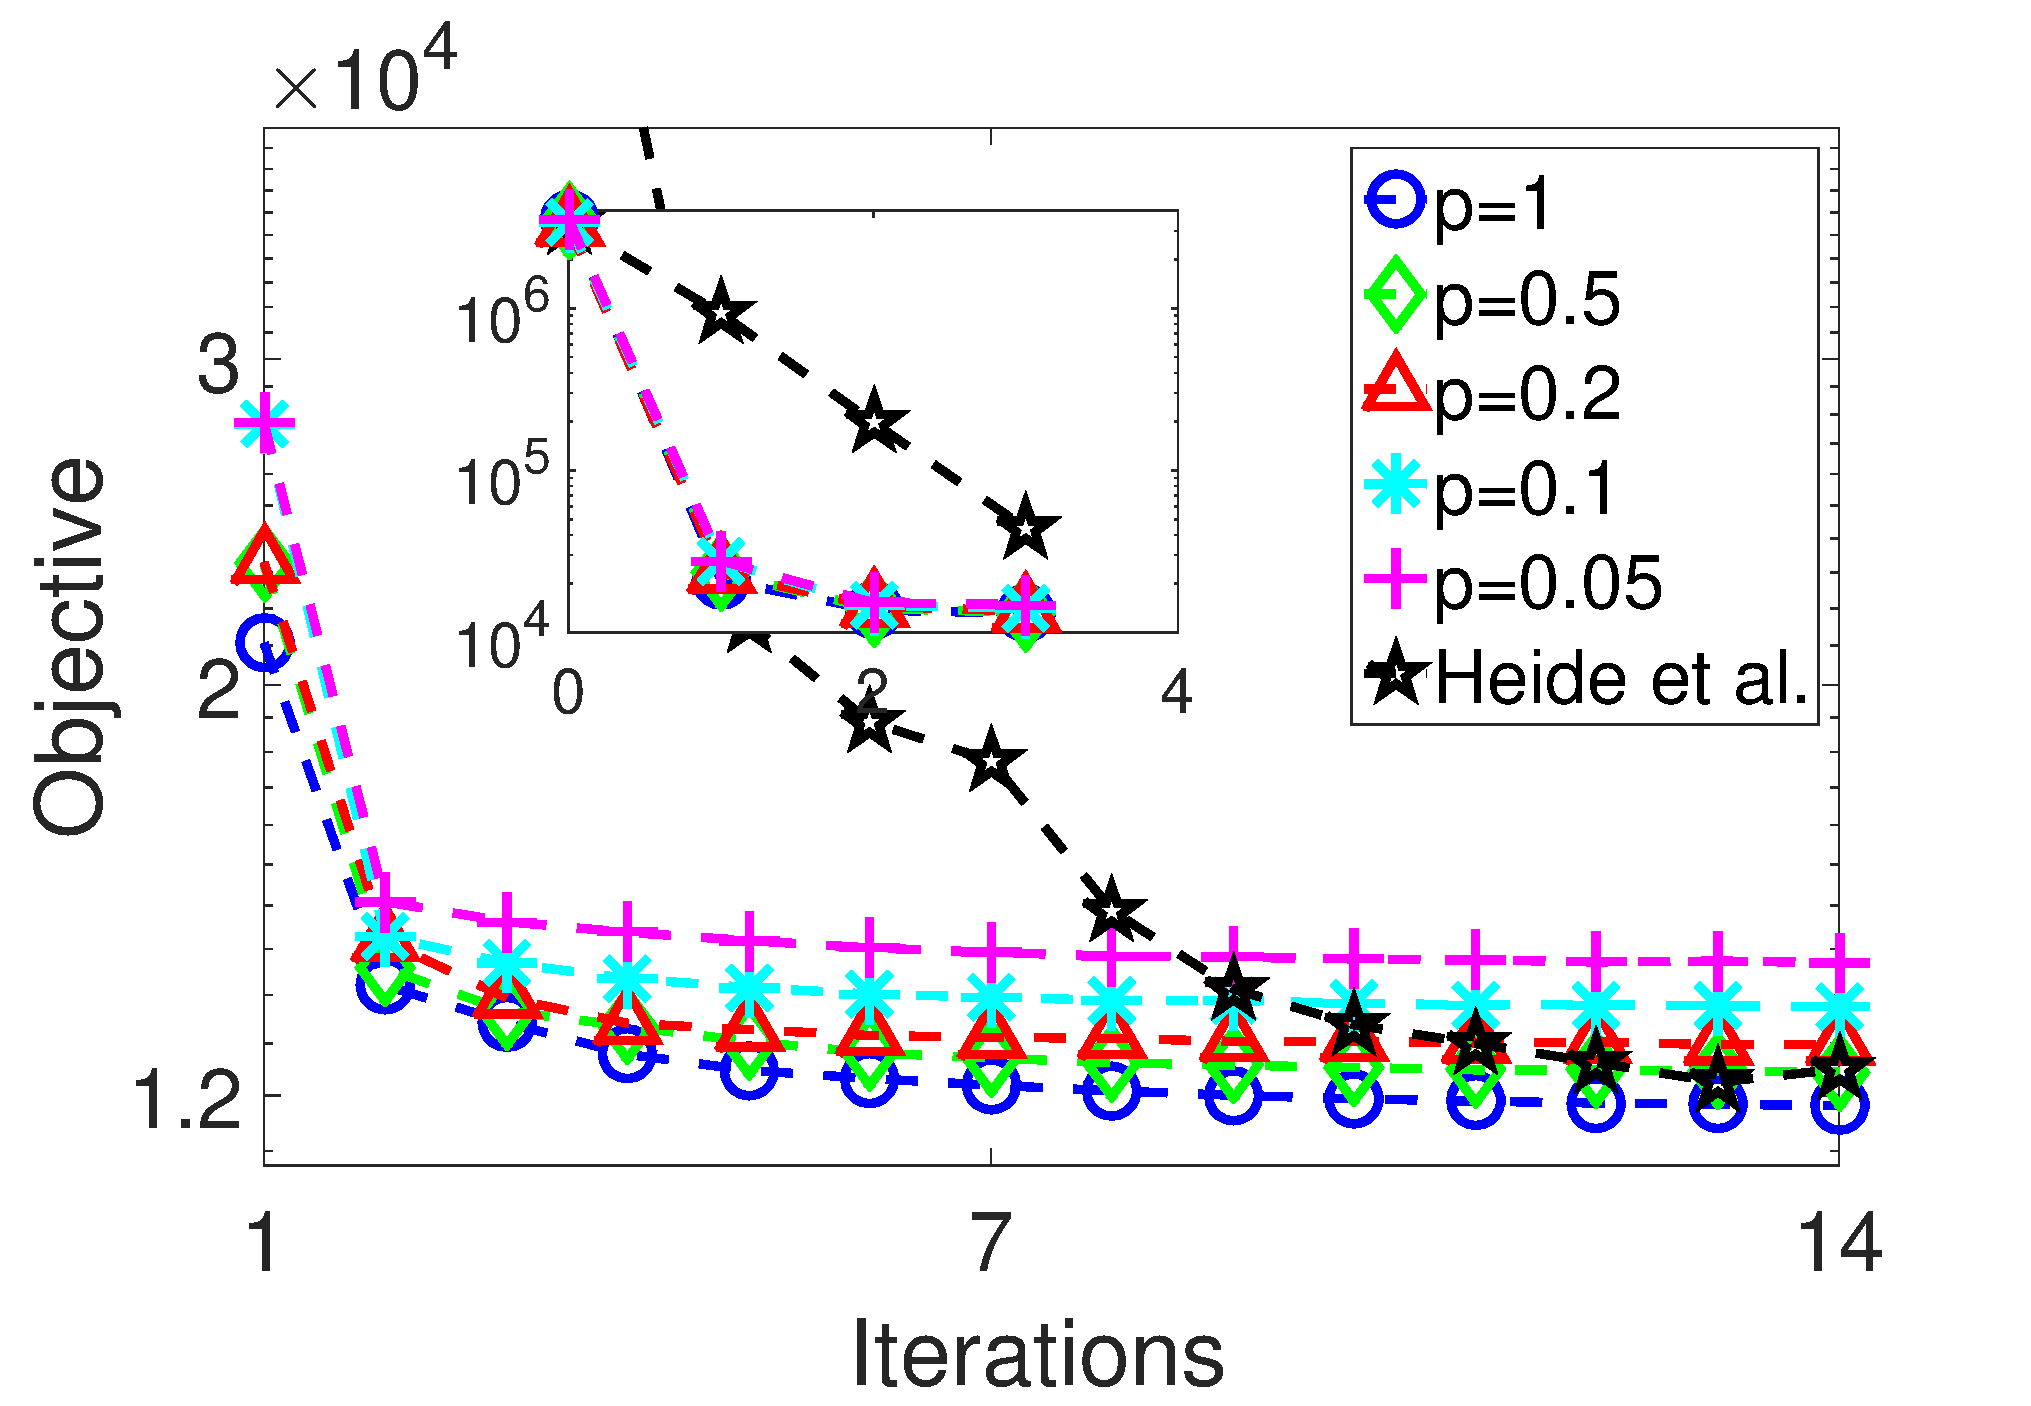
\includegraphics[width=1\linewidth]{figure/iteVSobj.pdf}
\end{subfigure}

\begin{subfigure}{0.5\textwidth}
  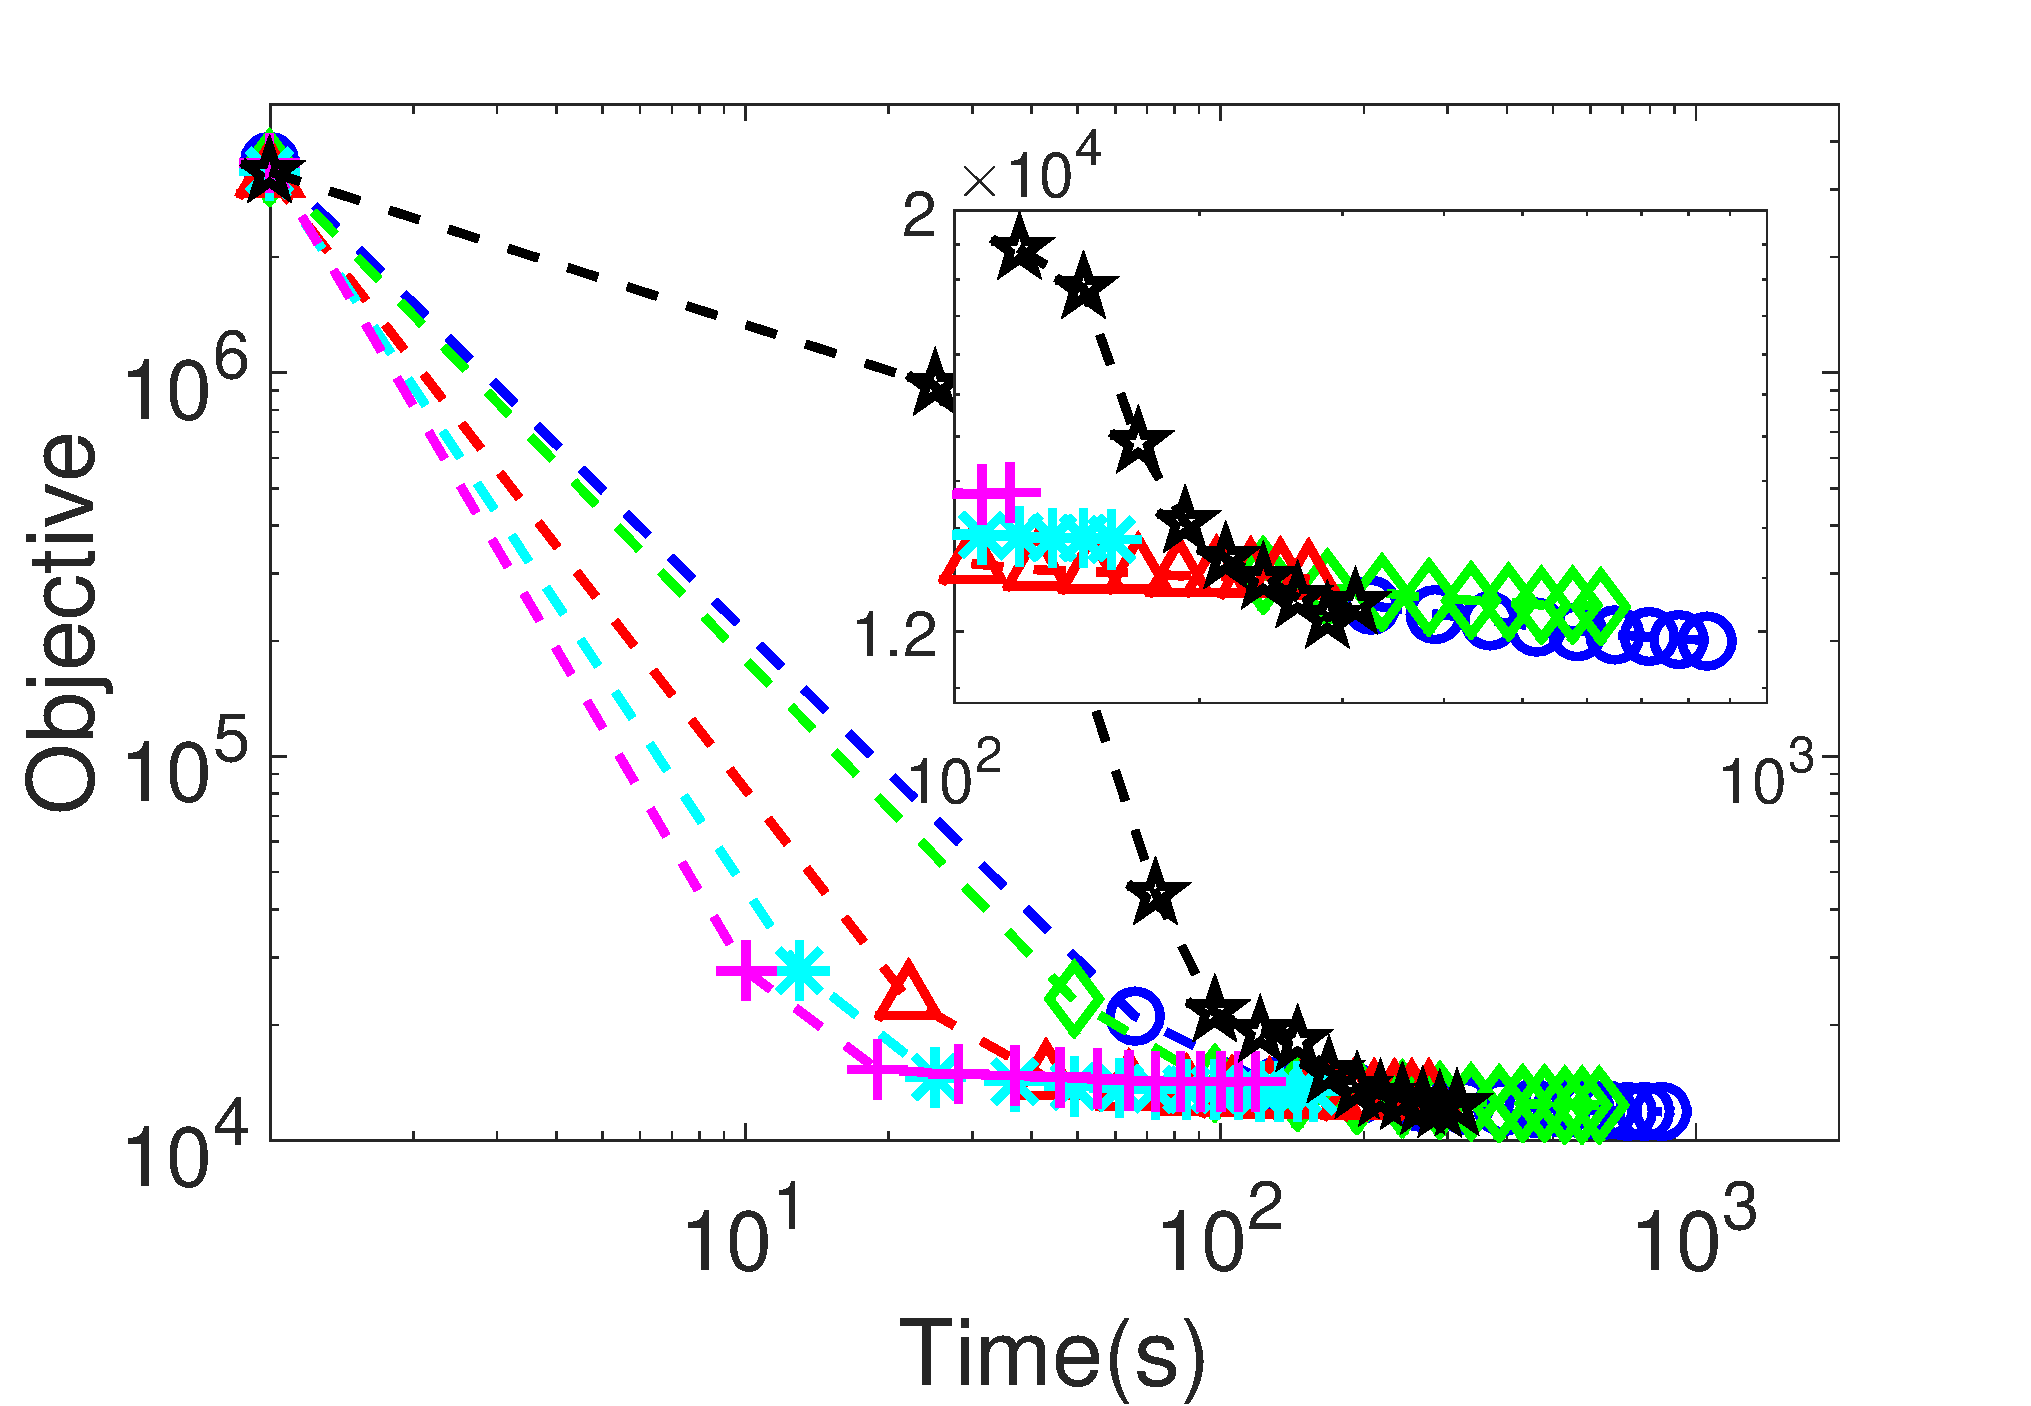
\includegraphics[width=1\linewidth]{figure/timeVSobj.pdf}
\end{subfigure}

\begin{subfigure}{0.23\textwidth}
  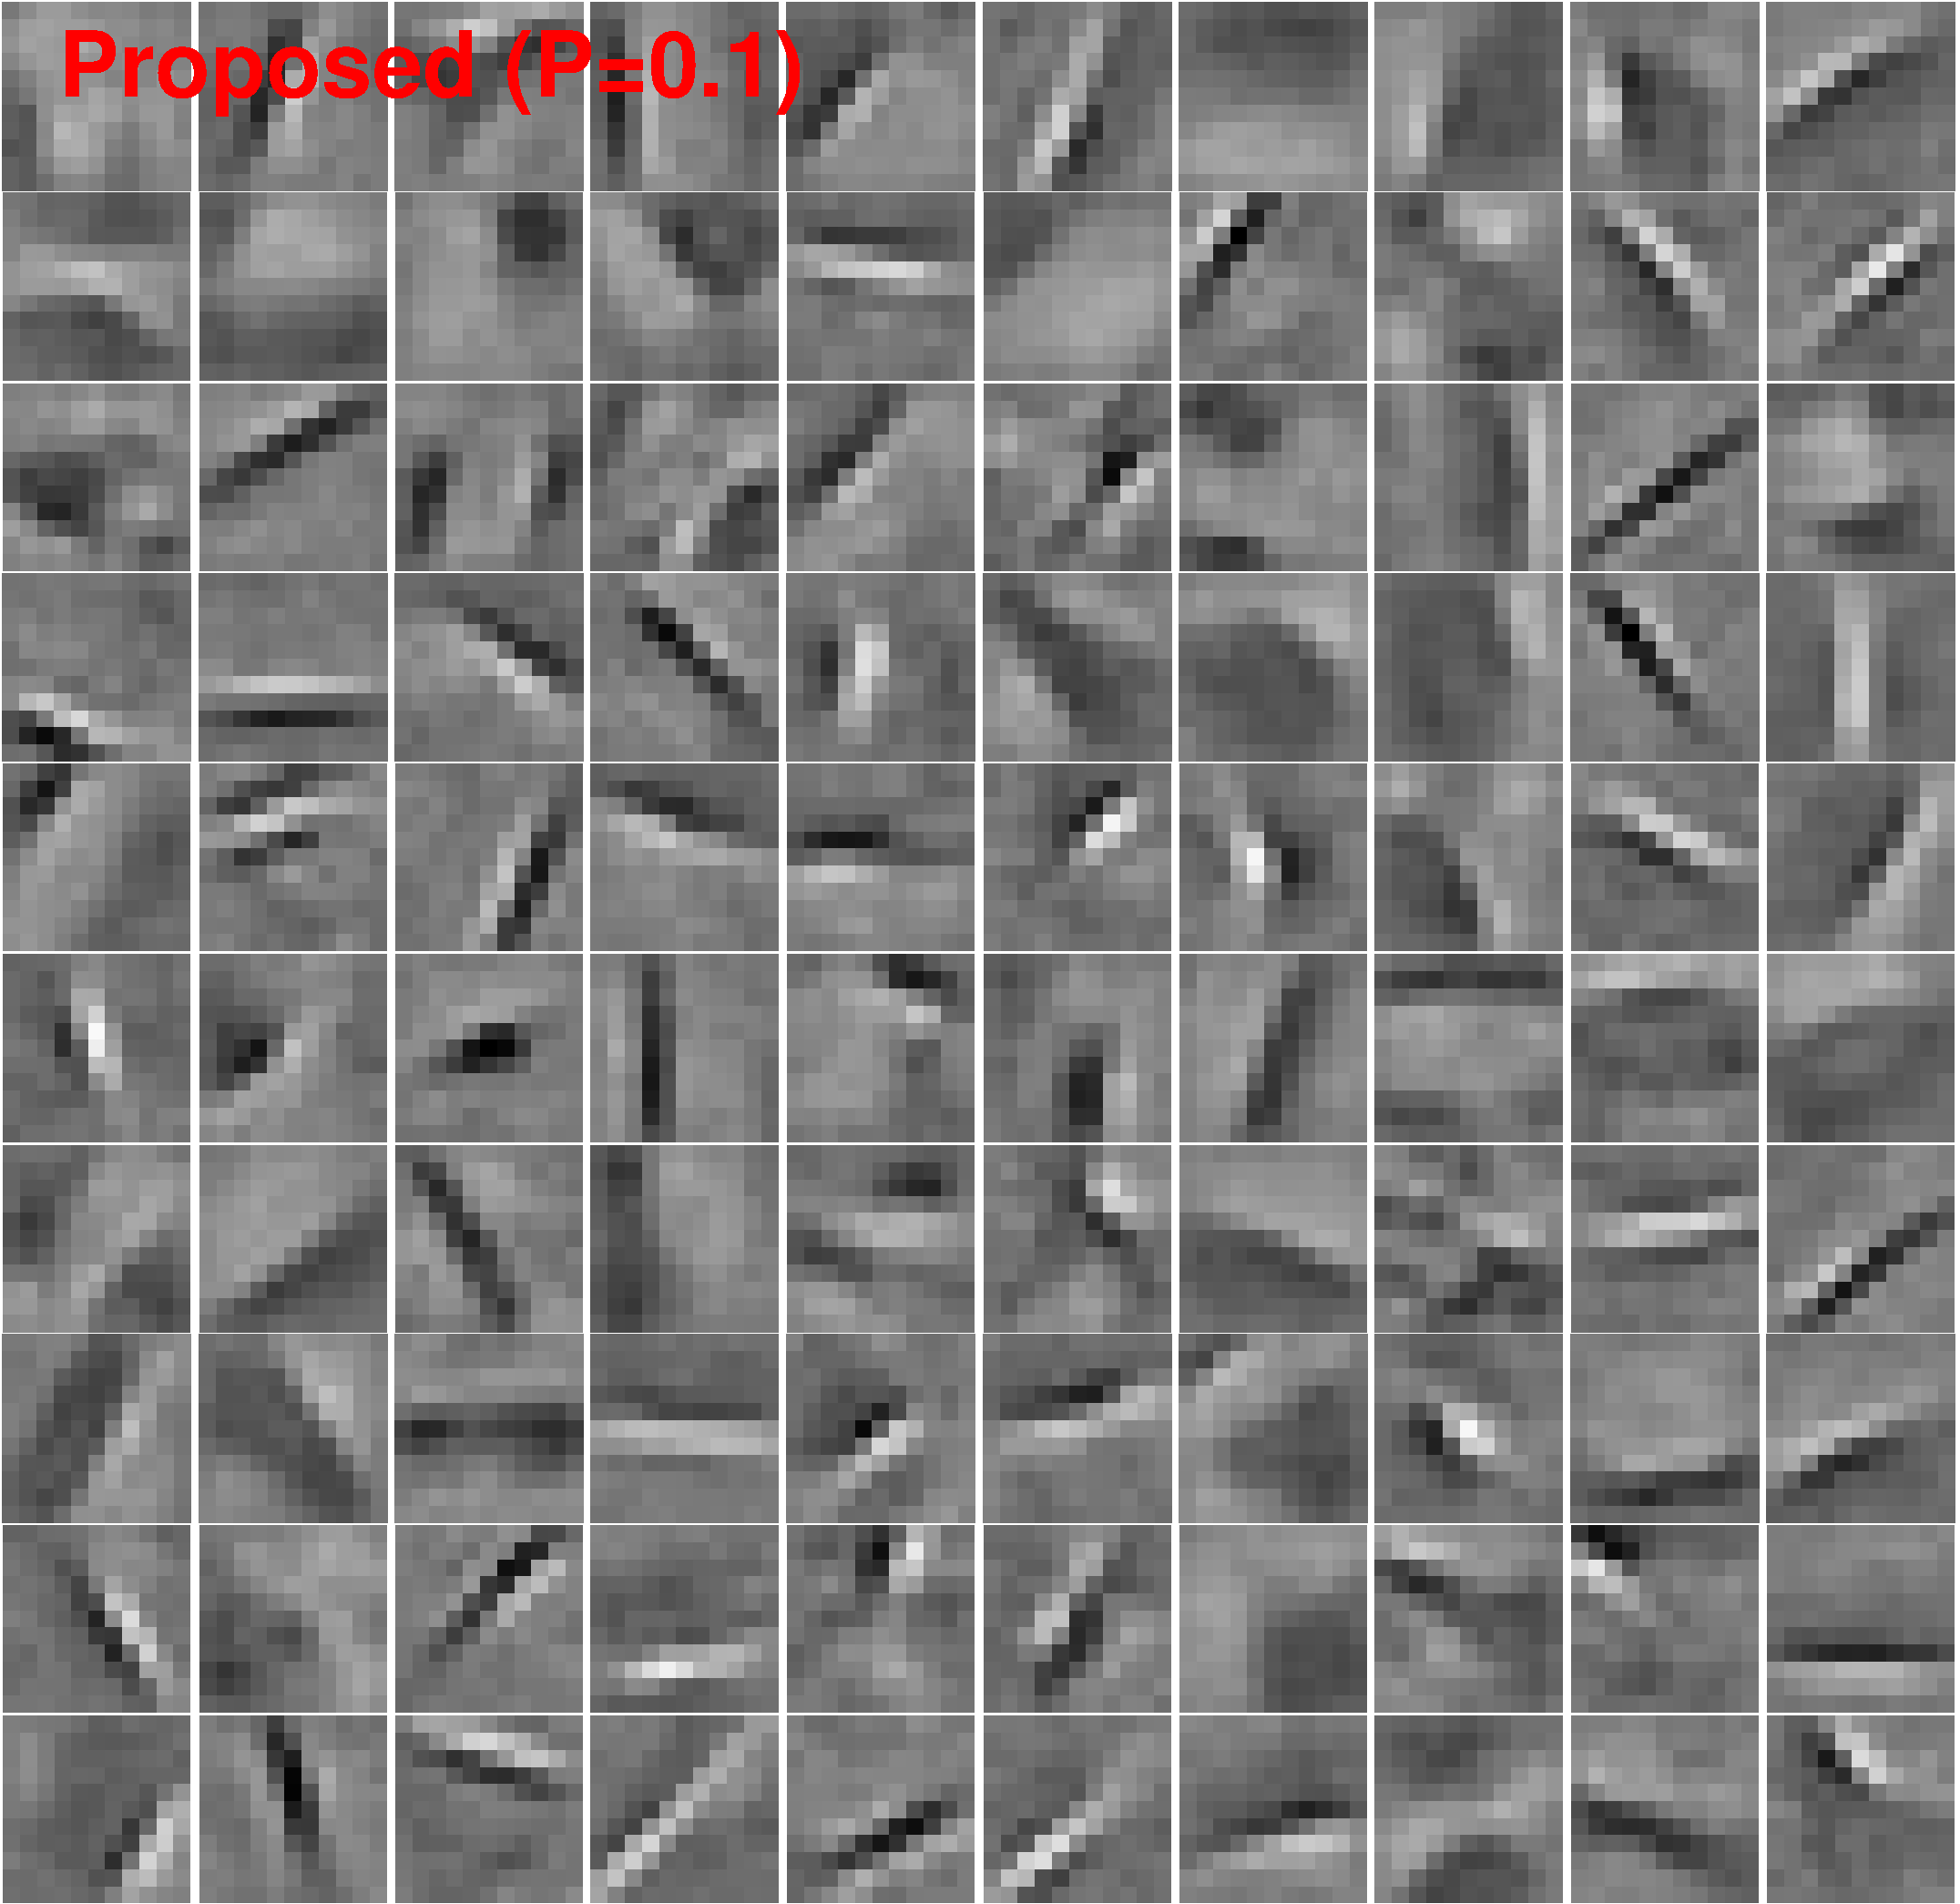
\includegraphics[width=1\linewidth]{figure/batchFruit100.pdf}
\end{subfigure}
\begin{subfigure}{0.23\textwidth}
  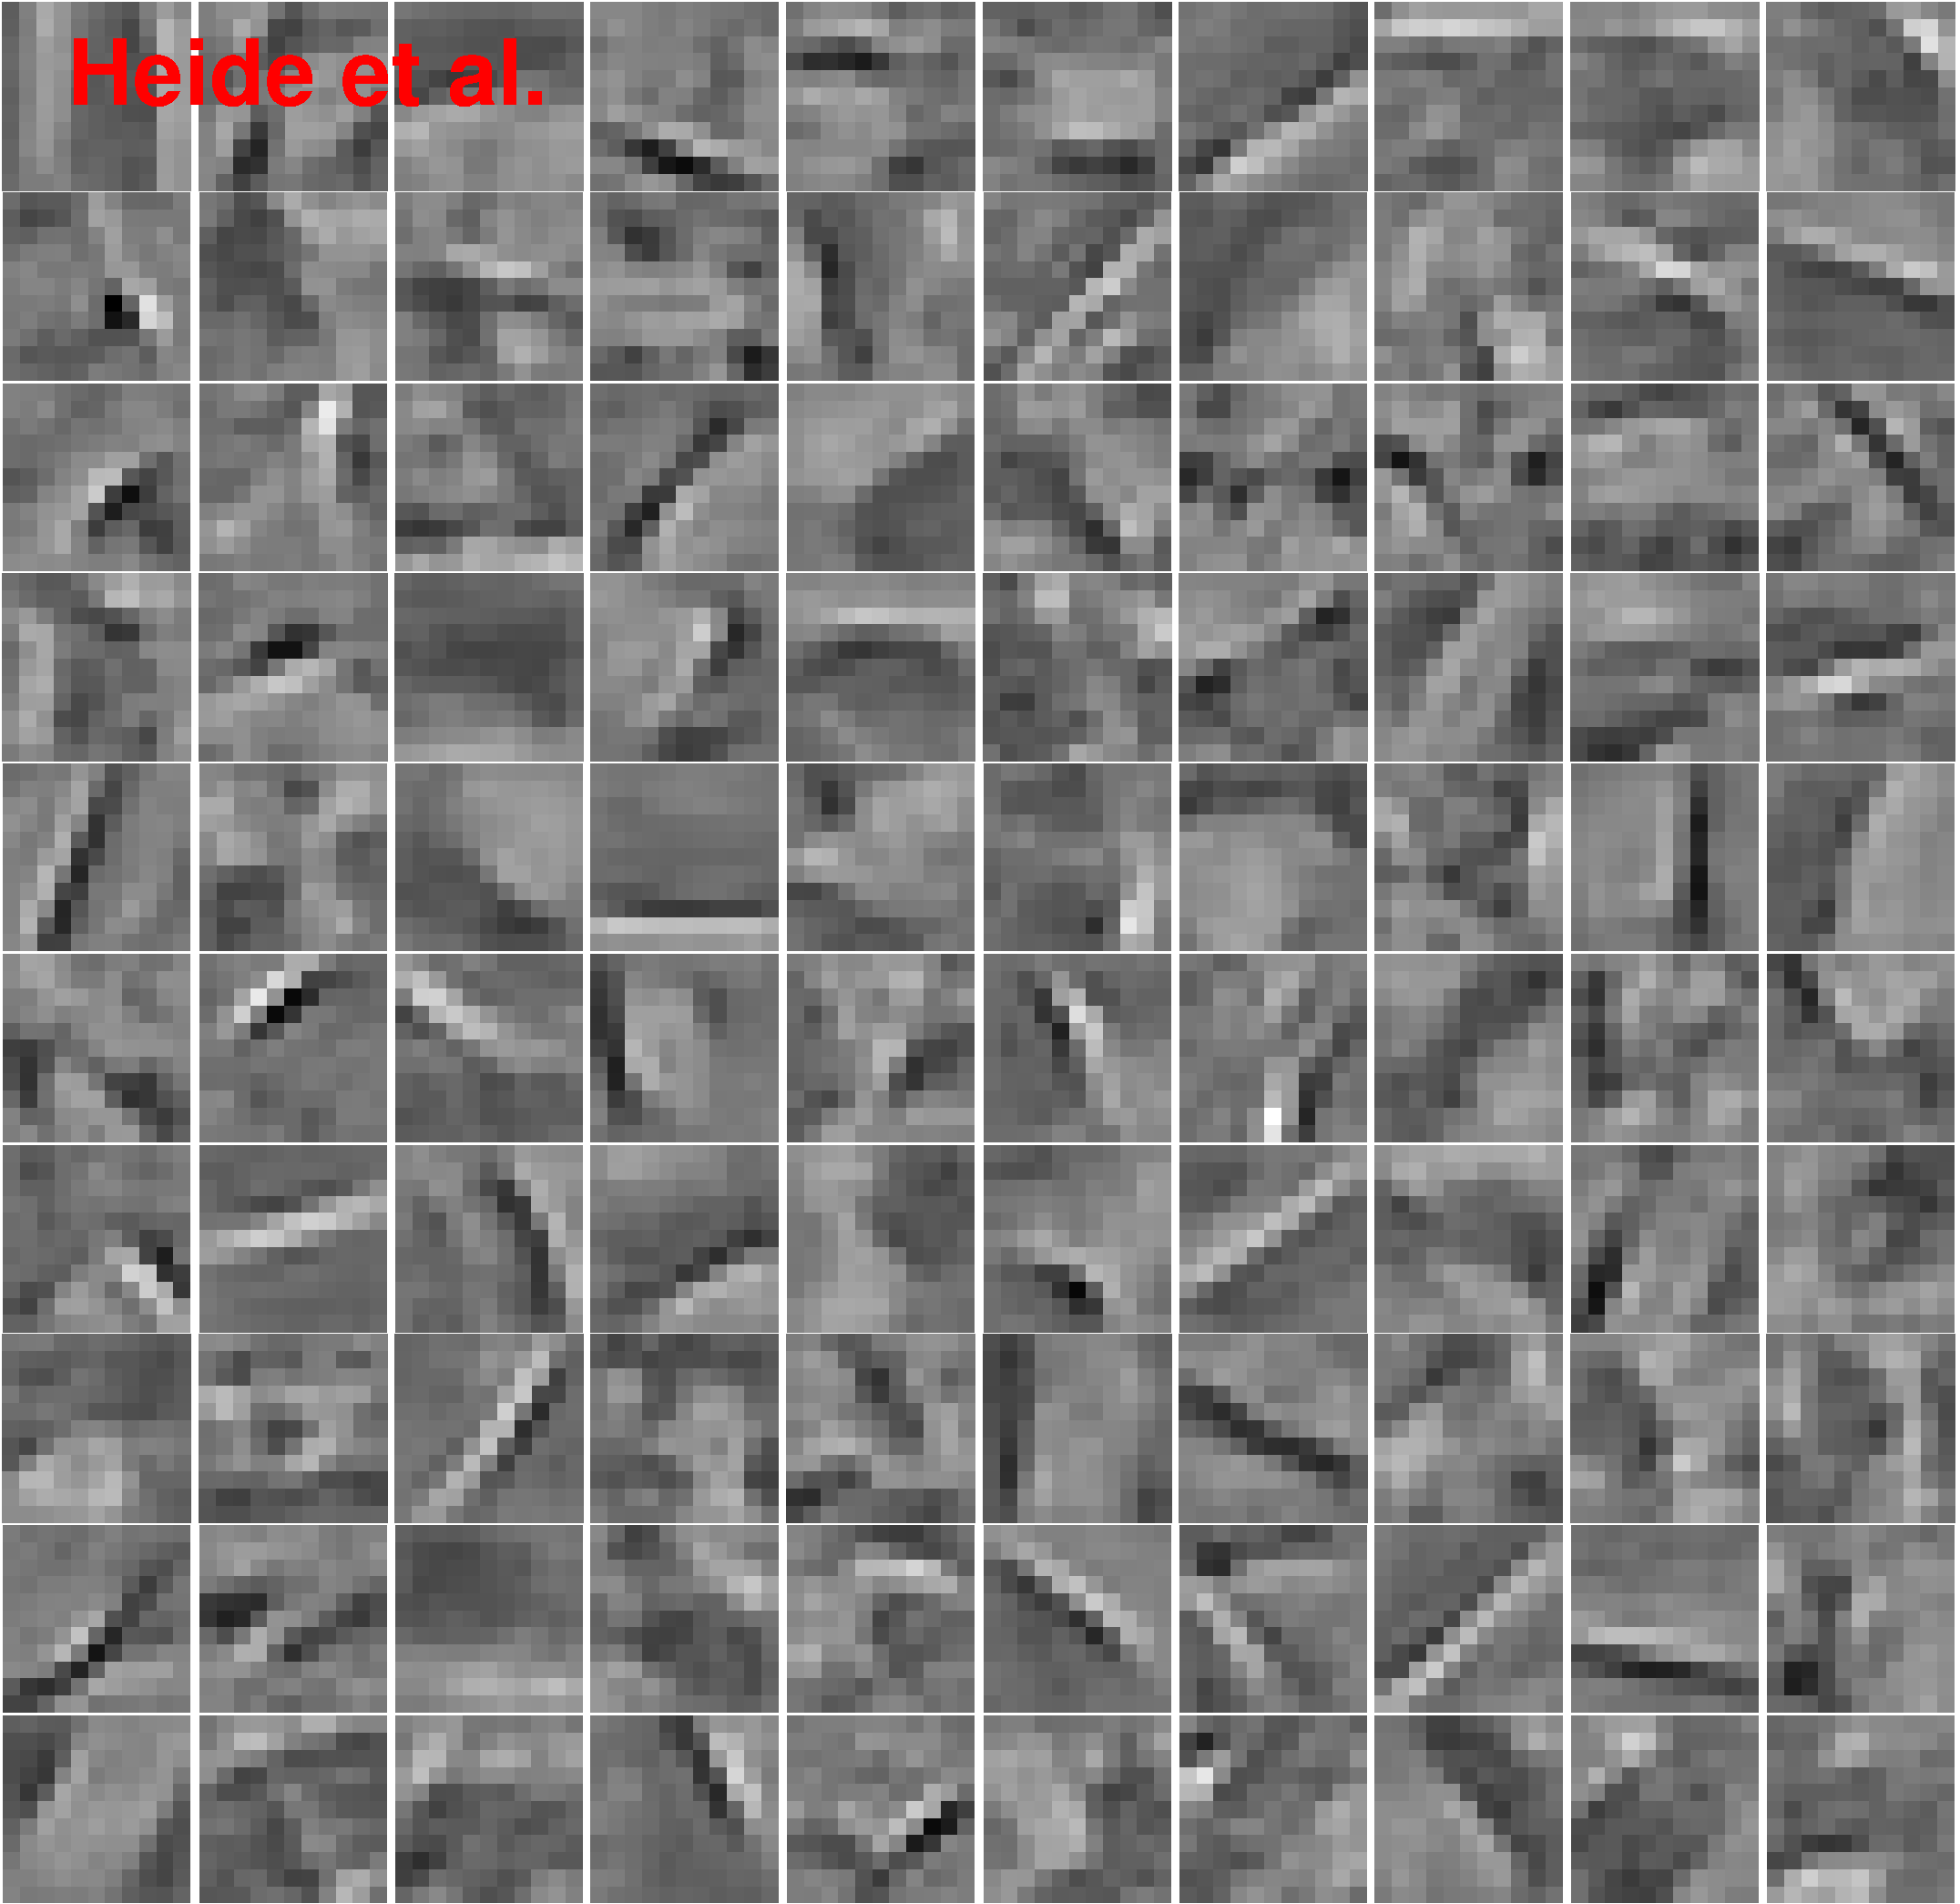
\includegraphics[width=1\linewidth]{figure/heideFruit100.pdf}
\end{subfigure}

\caption{Top: Convergence comparison between the-state-of-art method~\cite{heide2015fast} and the proposed method with different subsampling rate, all of which on performed on fruit dataset. Convergence is evaluated by monitoring the objective value of eq.~\ref{eq:CSCmodel} on training images versus iterations and time, respectively. Bottom: Learned filters by the proposed method with $p=0.1$ and the comparable method. In these represented learned filters, our method learns more smooth Gabor-like filters and less number of noise-like filters with the same $\lambda$. Beyond this, it runs faster with regard to each iteration and shows better convergence behavior.}
\label{fig:subsampleResult}
\end{figure}

\begin{figure*}[h]
    \centering
    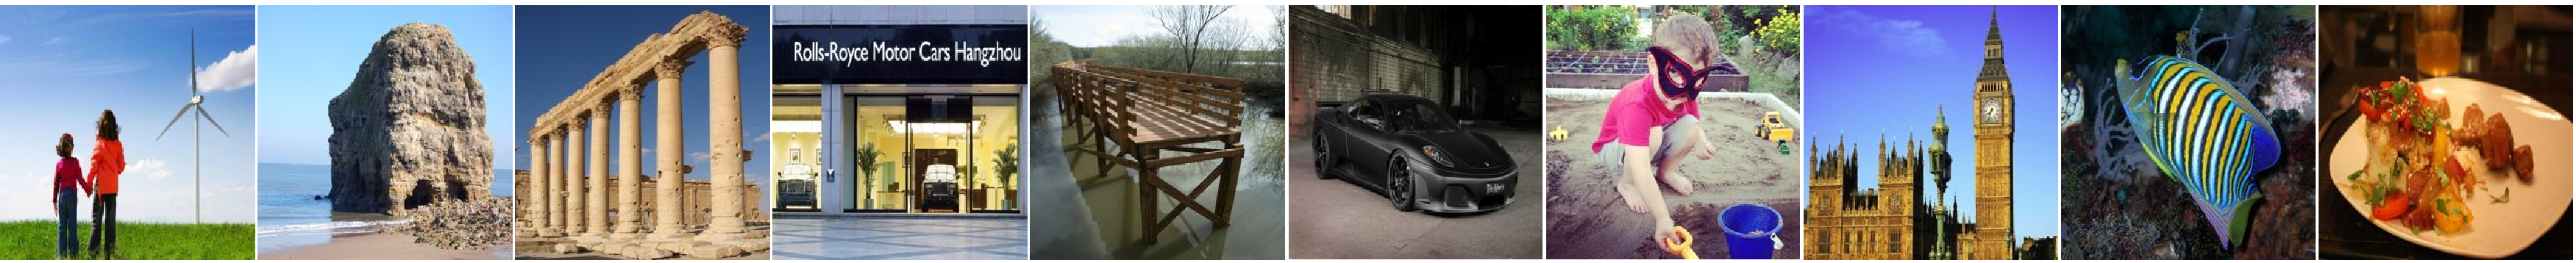
\includegraphics[width=1\textwidth]{figure/reconImage.pdf}
    \resizebox{0.9\linewidth}{!}{
        \begin{tabular}{|c||c|c|c|c|c|c|c|c|c|c|}
            \cline{1-11}
            Image & 1 & 2 & 3 & 4 & 5 & 6 & 7 & 8 & 9 & 10 \\
            \hline
            PSNR~\cite{heide2015fast} & 29.54 & 28.16 & 29.40 & 29.22 & 28.89 & 29.29 & 28.10  & 29.57 & 27.46 & 30.72 \\
            \hline
            PSNR ours & \textbf{29.65} & \textbf{28.18} & \textbf{29.52} & \textbf{29.43} & \textbf{28.99} & \textbf{29.38} & \textbf{28.19} & \textbf{29.63} & \textbf{27.62} & \textbf{30.98} \\
            \hline
        \end{tabular} }
    \caption{Numerical comparisons of the reconstruction quality obtained from the presented filters and its comparison. The reconstructions are performed on $50\%$ randomly observed images, with $\lambda = 0.4$ and $50$ ADMM iterations for both cases. Obtained PSNR values are averaged on 5 trials. Note that none of the testing images are in the training sets.} \label{fig:PSNRrecon}
\end{figure*}

\subsection{Subsampling Strategy}

{\bfseries Convergence.} Comparisons of the convergence between the proposed method (SBCSC) and the state-of-the-art batch-mode algorithm~\cite{heide2015fast} are shown in Fig.\ \ref{fig:subsampleResult}. A different selection of the subsampling rate reveals that the proposed strategy will slightly influence the convergence and the training objective of the minimization problem. Specifically, the more subsampled, the relatively slower convergence and the higher objective will be obtained. On the other hand, small subsampling rate will significantly accelerate the computation process, where $10\%$ subsampling achieves about $6 \times$ speedup over no subsampled solver and $2 \times$ speedup over state-of-the-art frequency solver for one iteration. We observe that a subsampling rate between $0.1$ and $0.2$ delivers empirically good enough convergence in our settings, as well as achieving at least $3 \times$ speedup. In general, the proposed method with various subsampling rates converges at around 10-12 iterations in all testing cases, acting similar to the competing methods. Notice that the comparable method has a relatively high objective at first $6-8$ iterations due to different splitting strategies are applied and subproblems are interleaved on the primary variables~\cite{wohlberg2016efficient}, though it converges to an optimum with comparable objective after 10 iterations. In summary, comparing to the state-of-the-art frequency solver, the proposed stochastic spatial-domain solver with a subsampling rate $10\%$ reduces the computation time by a factor of two for the tested example. Please see supplementary materials for additional experimental results.

{\bfseries Reconstruction}. The learned filters by SBCSC with subsampling rate $0.1$ are shown in the bottom of Fig.\ \ref{fig:subsampleResult}. For a visual comparison, we also show the filters learned from the competing method (bottom left of Figure 3 in~\cite{heide2015fast}. As can be observed, both of them learn some seemingly similar Gabor-like filters. While after zooming (we also show zoom-in comparisons in supplement), it can be seen that our learned Gabor-like filters have less impure structures. Moreover, the compared dictionary contains a number of noise-like filters, which are rarely existed in ours. We then demonstrate the effectiveness of the reconstructed filters in the application of image inpainting, which refers to reconstructing a full image from partial measurements. A numerical comparison of the reconstruction quality is shown in Fig.\ \ref{fig:PSNRrecon}. The filters learned by the proposed method not only show more visually decent structures and less specific features, but also demonstrate its capability to better reconstruct partial observed images with respect to the PSNR value. In addition to that, the learning process only takes about $50\%$ of the execution time than the comparison.

\subsection{Online Learning Settings}

{\bfseries Convergence.} Unlike the batch-based learning approaches which evaluate its convergence by monitoring the objective value on training datasets, a common way to evaluate the learning process of online learning model is to monitor its objective value on testing images. The testing objectives of the proposed method (SOCSC) and prior published online frequency-domain CSC method~\cite{liu-2018-first}, with respect to iterations, are shown in Fig.\ \ref{fig:onlineSmall}. In the same figure, we also keep track of the capability of the updated filters during the learning process to sparsely represent the testing images, which is demonstrated by the time evolution of PSNR. These two approaches stop at optimum positions with close testing objective values, though, they exhibit slightly different convergence behaviors with respect to iterations. The final testing PSNR values for both methods also reveal a similar reconstruction performance of the learned filters. As for the runtime comparison, the proposed method runs at least 5 times faster than the comparable method. Supplement shows additional comparisons for different datasets.

%The proposed method not only exhibits a better convergence performance, but also takes much less execution time, achieving roughly $5 \times$ speedup for one iteration. A visual comparison of the learned dictionaries also demonstrates that the proposed algorithm delivers better outcomes.
% Further numerical comparison will be reported in the next section.

{\bfseries Over-complete dictionary.} As far as we know, none of the precedent CSC work reported or analyzed the over-complete dictionary (the number of filters is more than the degrees of freedom). One of the reasons could be that most of the prior work is batch-based, thus learning over-complete dictionary from small datasets would cause the overfitting issue, which may contain quite a few data-specific filters, and therefore be short of the generalization ability (we verify this explanation in supplement). The proposed online-based learning strategy (SOCSC) can overcome this issue by scaling the model up to arbitrary sample sizes.

We demonstrate its capability on 1000 image patches with the size of $100 \times 100$, and learn $11 \times 11 \times 400$ over-complete dictionary, all of which are shown in Fig.\ \ref{fig:overCompleteDic} . For a visual comparison, 100 learned filters by the same algorithm and its comparable approach~\cite{liu-2018-first} are also represented. As can be observed, both of the approaches learn visually similar under-complete dictionary, while the proposed method takes $5 \times$ less training time than the competitive one. As for the learned over-complete dictionary, it is composed of the Gabor-like image features as represented in the under-complete dictionaries, as well as a number of low contrast features which are rarely existed in those under-complete dictionaries. This additional feature information would play an essential role to better reconstruct the natural images, which can be demonstrated by the results of reconstruction quality shown in the same figure.

We further show a bottleneck revealed by the under-complete dictionary in the online-based CSC model. The top of Fig.\ \ref{fig:overComDicAndMinibatch} demonstrates that no more apparent progress could be observed when the number of training images is higher than a specific value for both of the online approaches ($K=100$). However, owing to more abundant filters, learning over-complete dictionary overcomes this bottleneck, and it shows a considerable improvement, with regard to PSNR, to have a sparse representation of the testing images during the learning process. This is also verified by applying these learned dictionaries to the image inpainting application as discussed above.

\begin{figure}[h]
\centering
\begin{subfigure}{0.49\textwidth}
  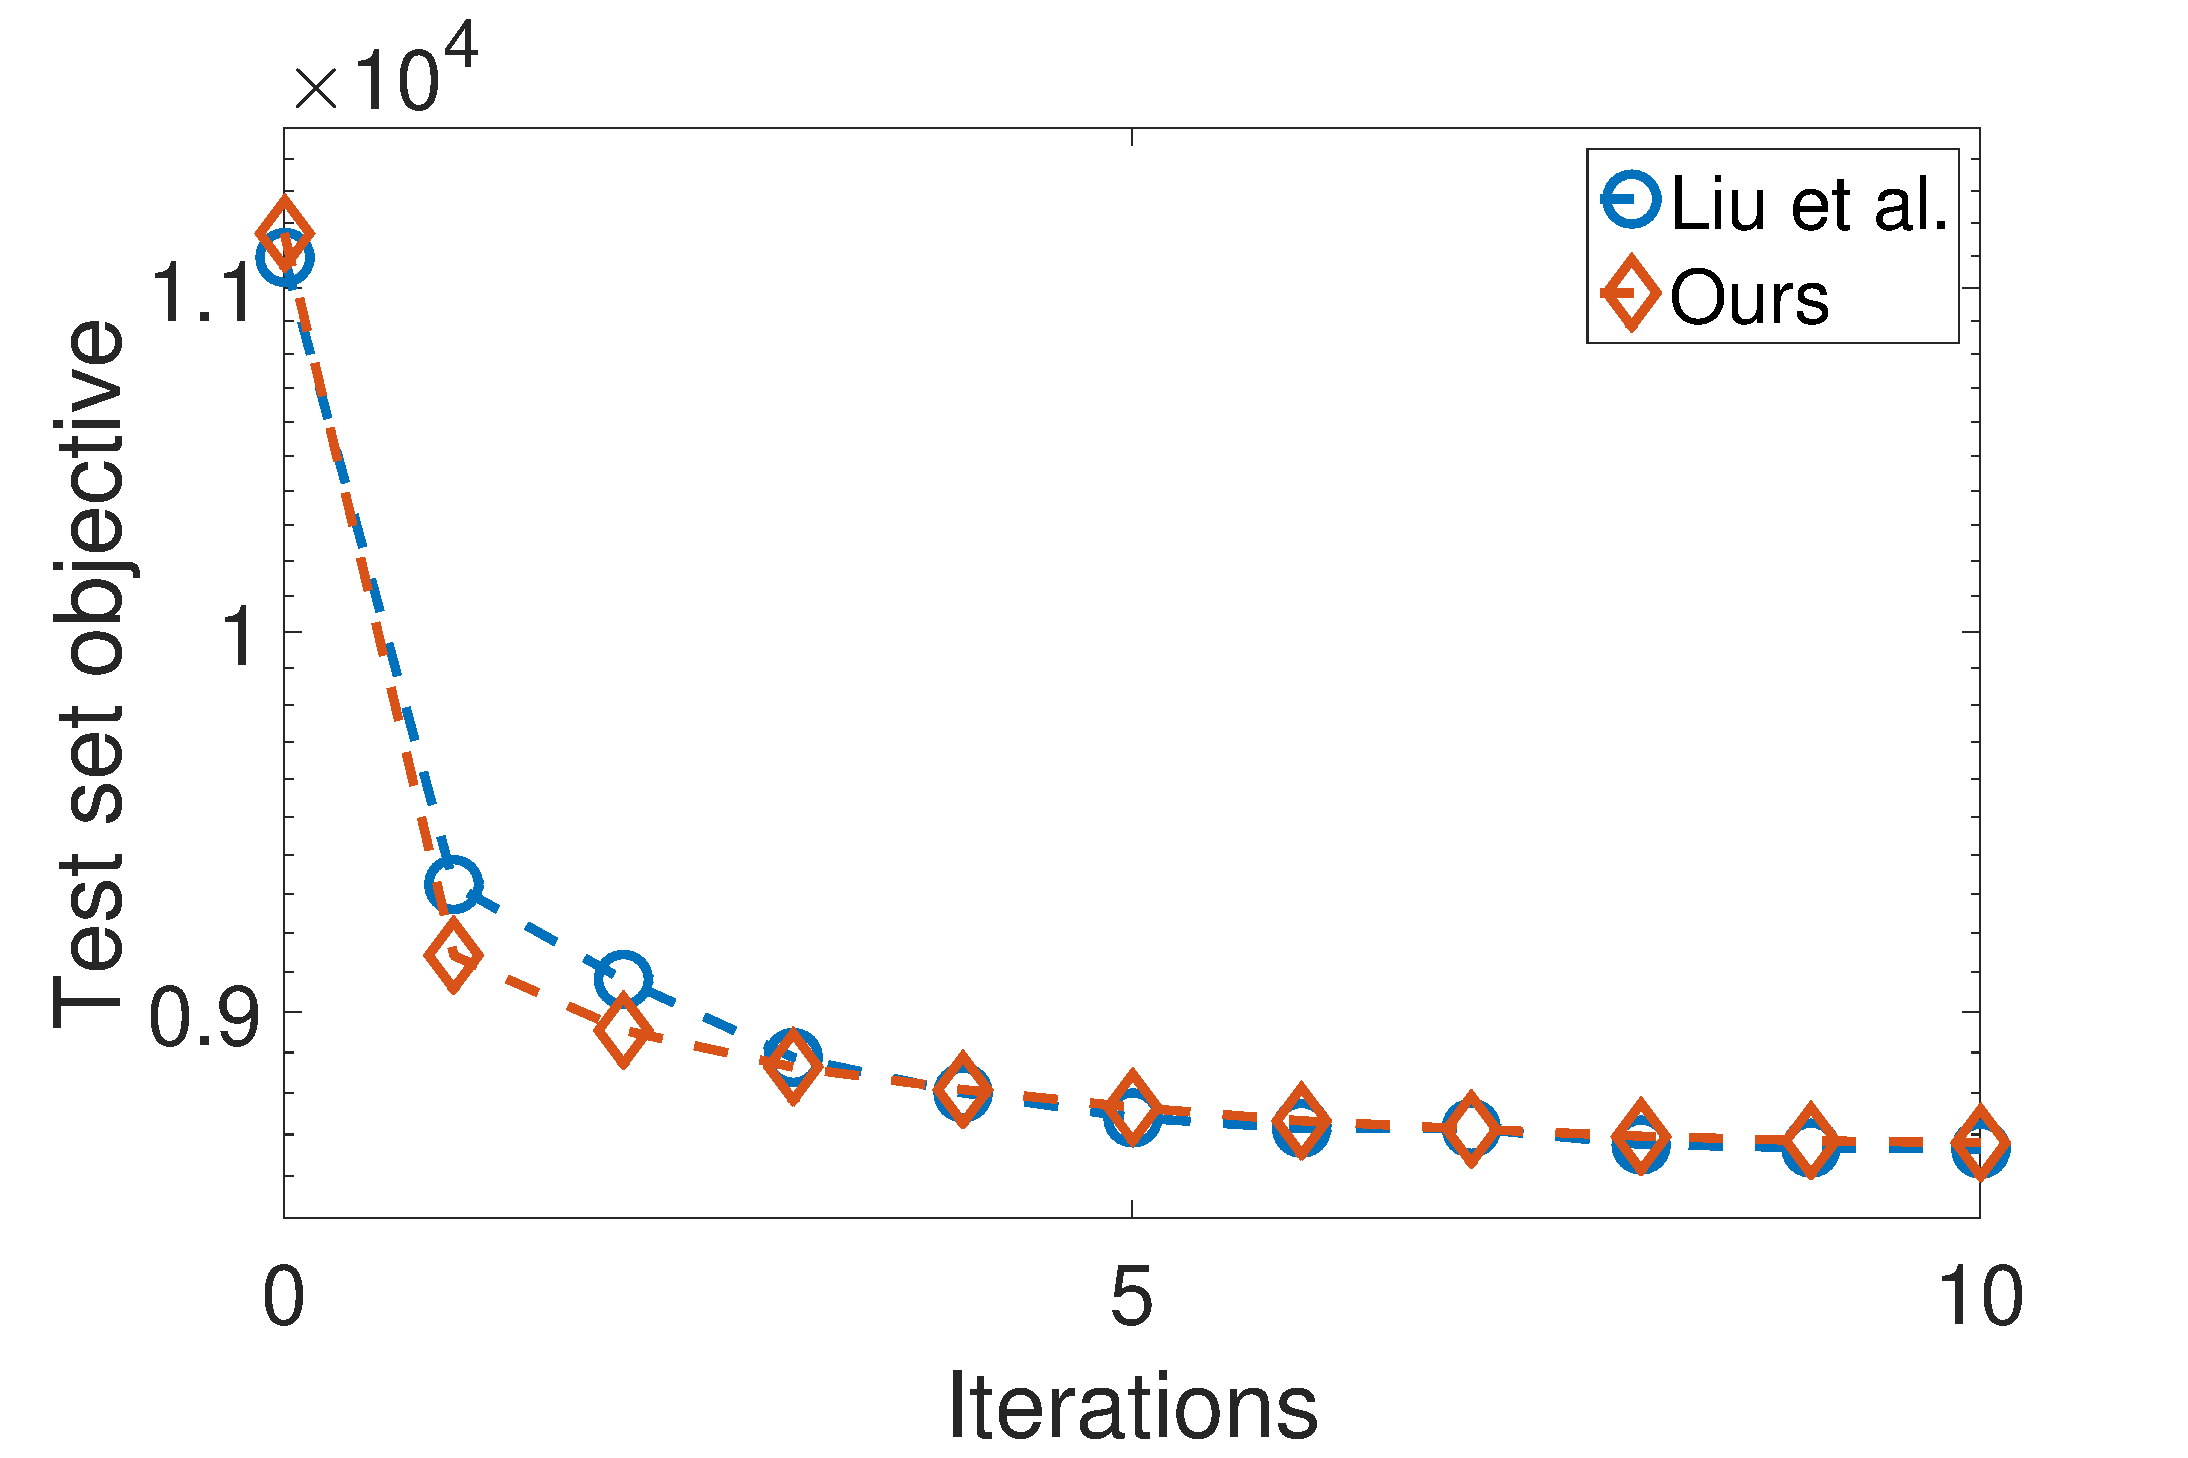
\includegraphics[width=1\linewidth]{figure/onlineVSliu-ite-fruit.pdf}
\end{subfigure}
\begin{subfigure}{0.49\textwidth}
  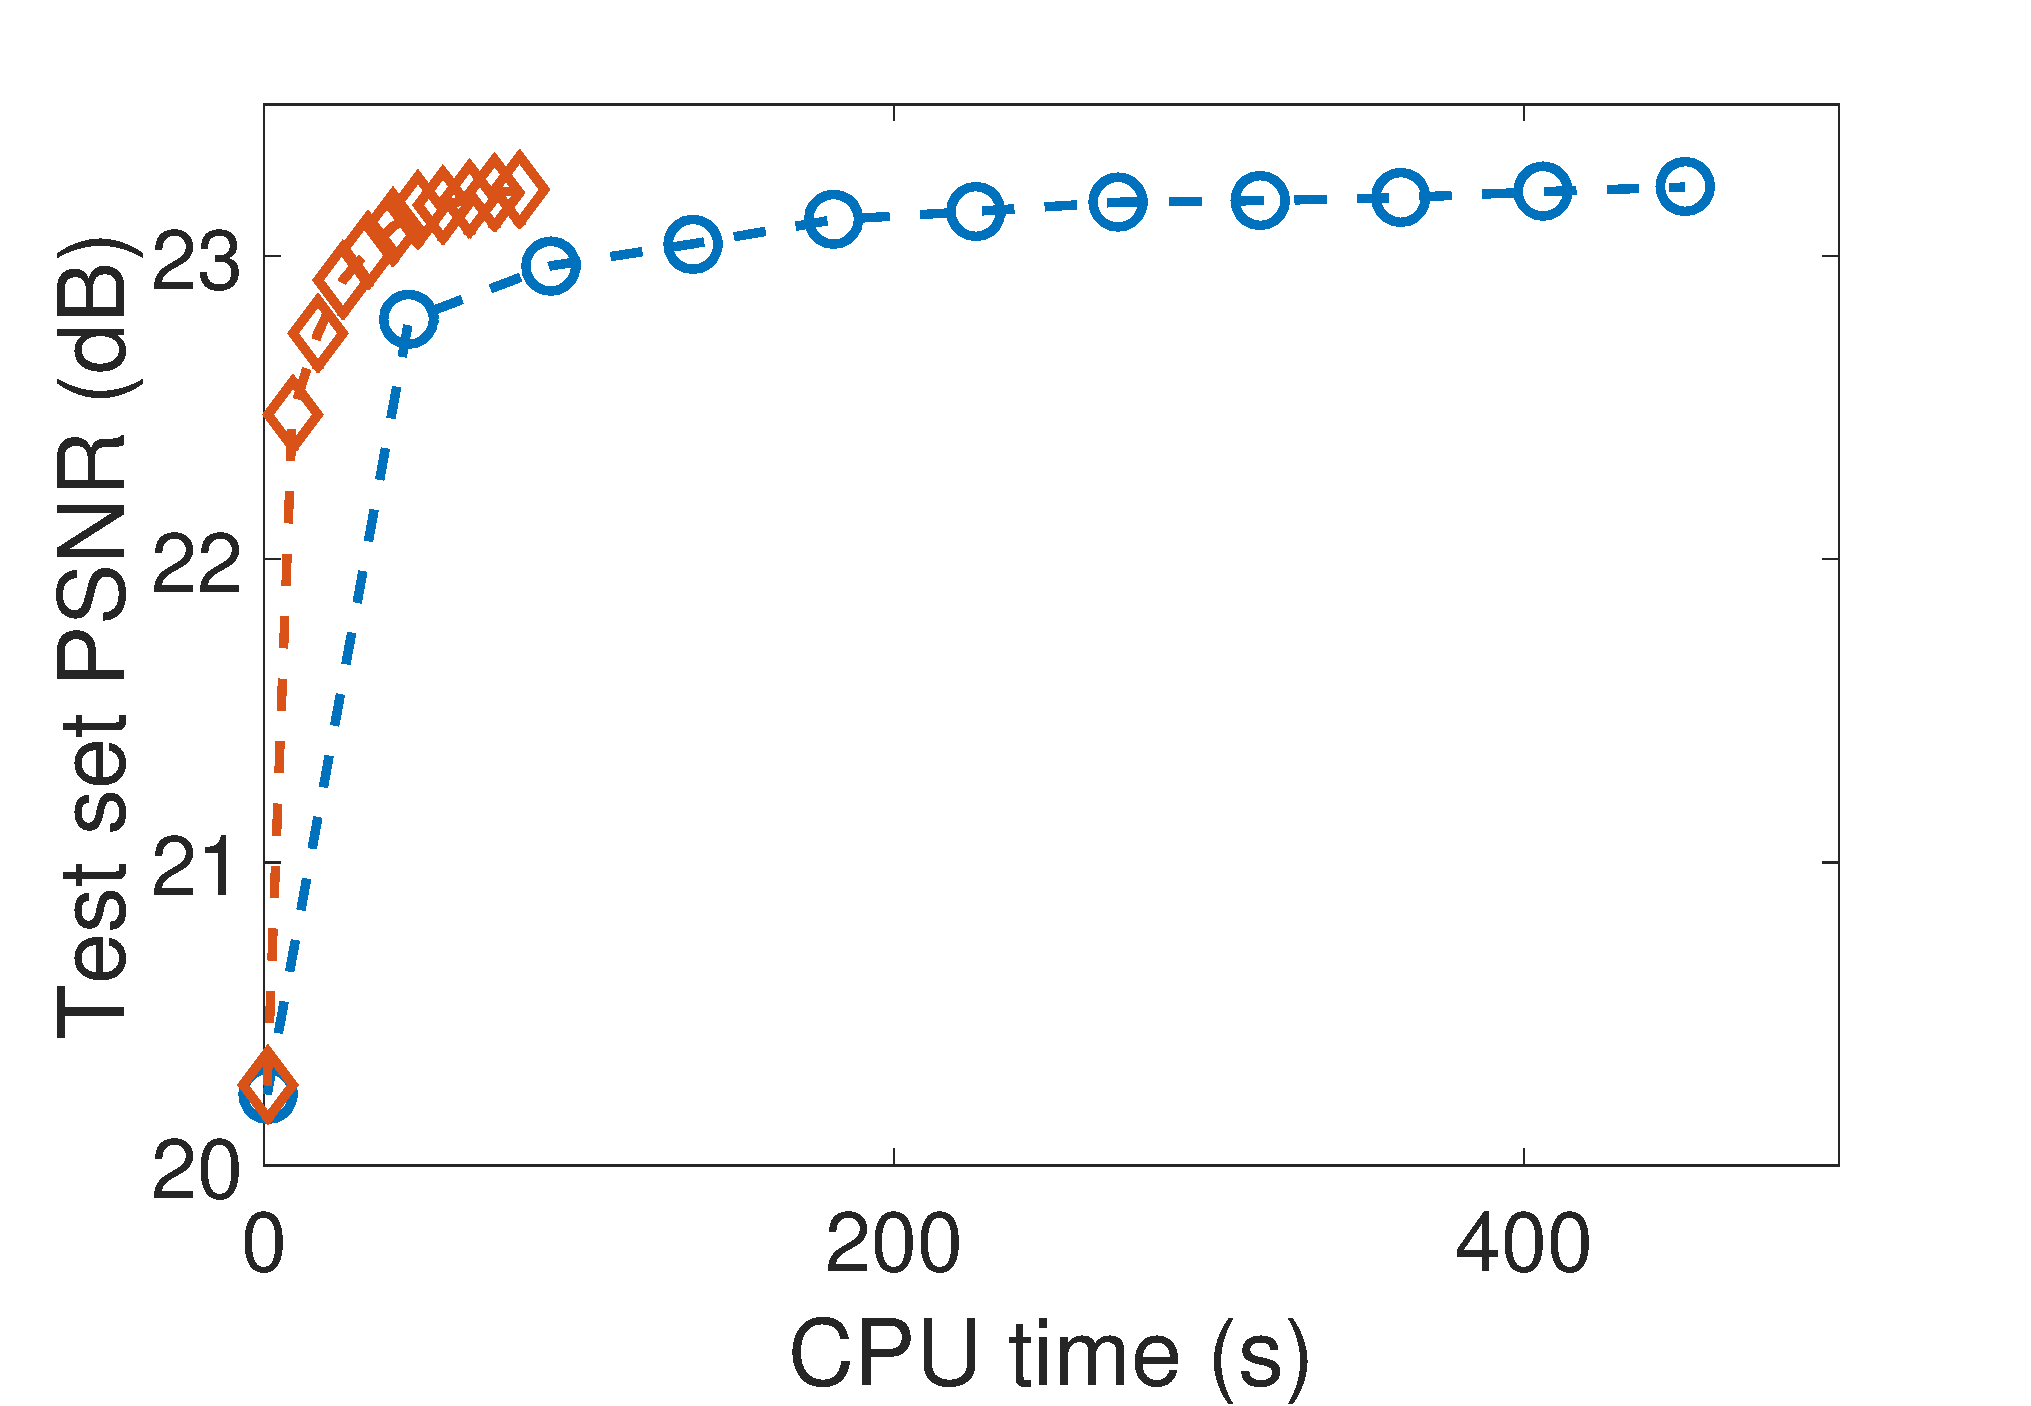
\includegraphics[width=1\linewidth]{figure/onlineVSliu-time-fruit.pdf}
\end{subfigure}

\caption{The experiments are performed on fruit dataset, and each iteration randomly choose one image from the training sets. Top: Convergence of the test set objectives for our method (SOCSC) and the state-of-the-art online approach~\cite{liu-2018-first}. Bottom: Testing PSNR with respect to execution time. While the quality of the output is comparable, our method achieves $5 \times$ speedup.}
\label{fig:onlineSmall}
\end{figure}

\begin{figure*}[h]
\begin{minipage}{0.4\textwidth}
\begin{subfigure}{1\textwidth}
    \centering
  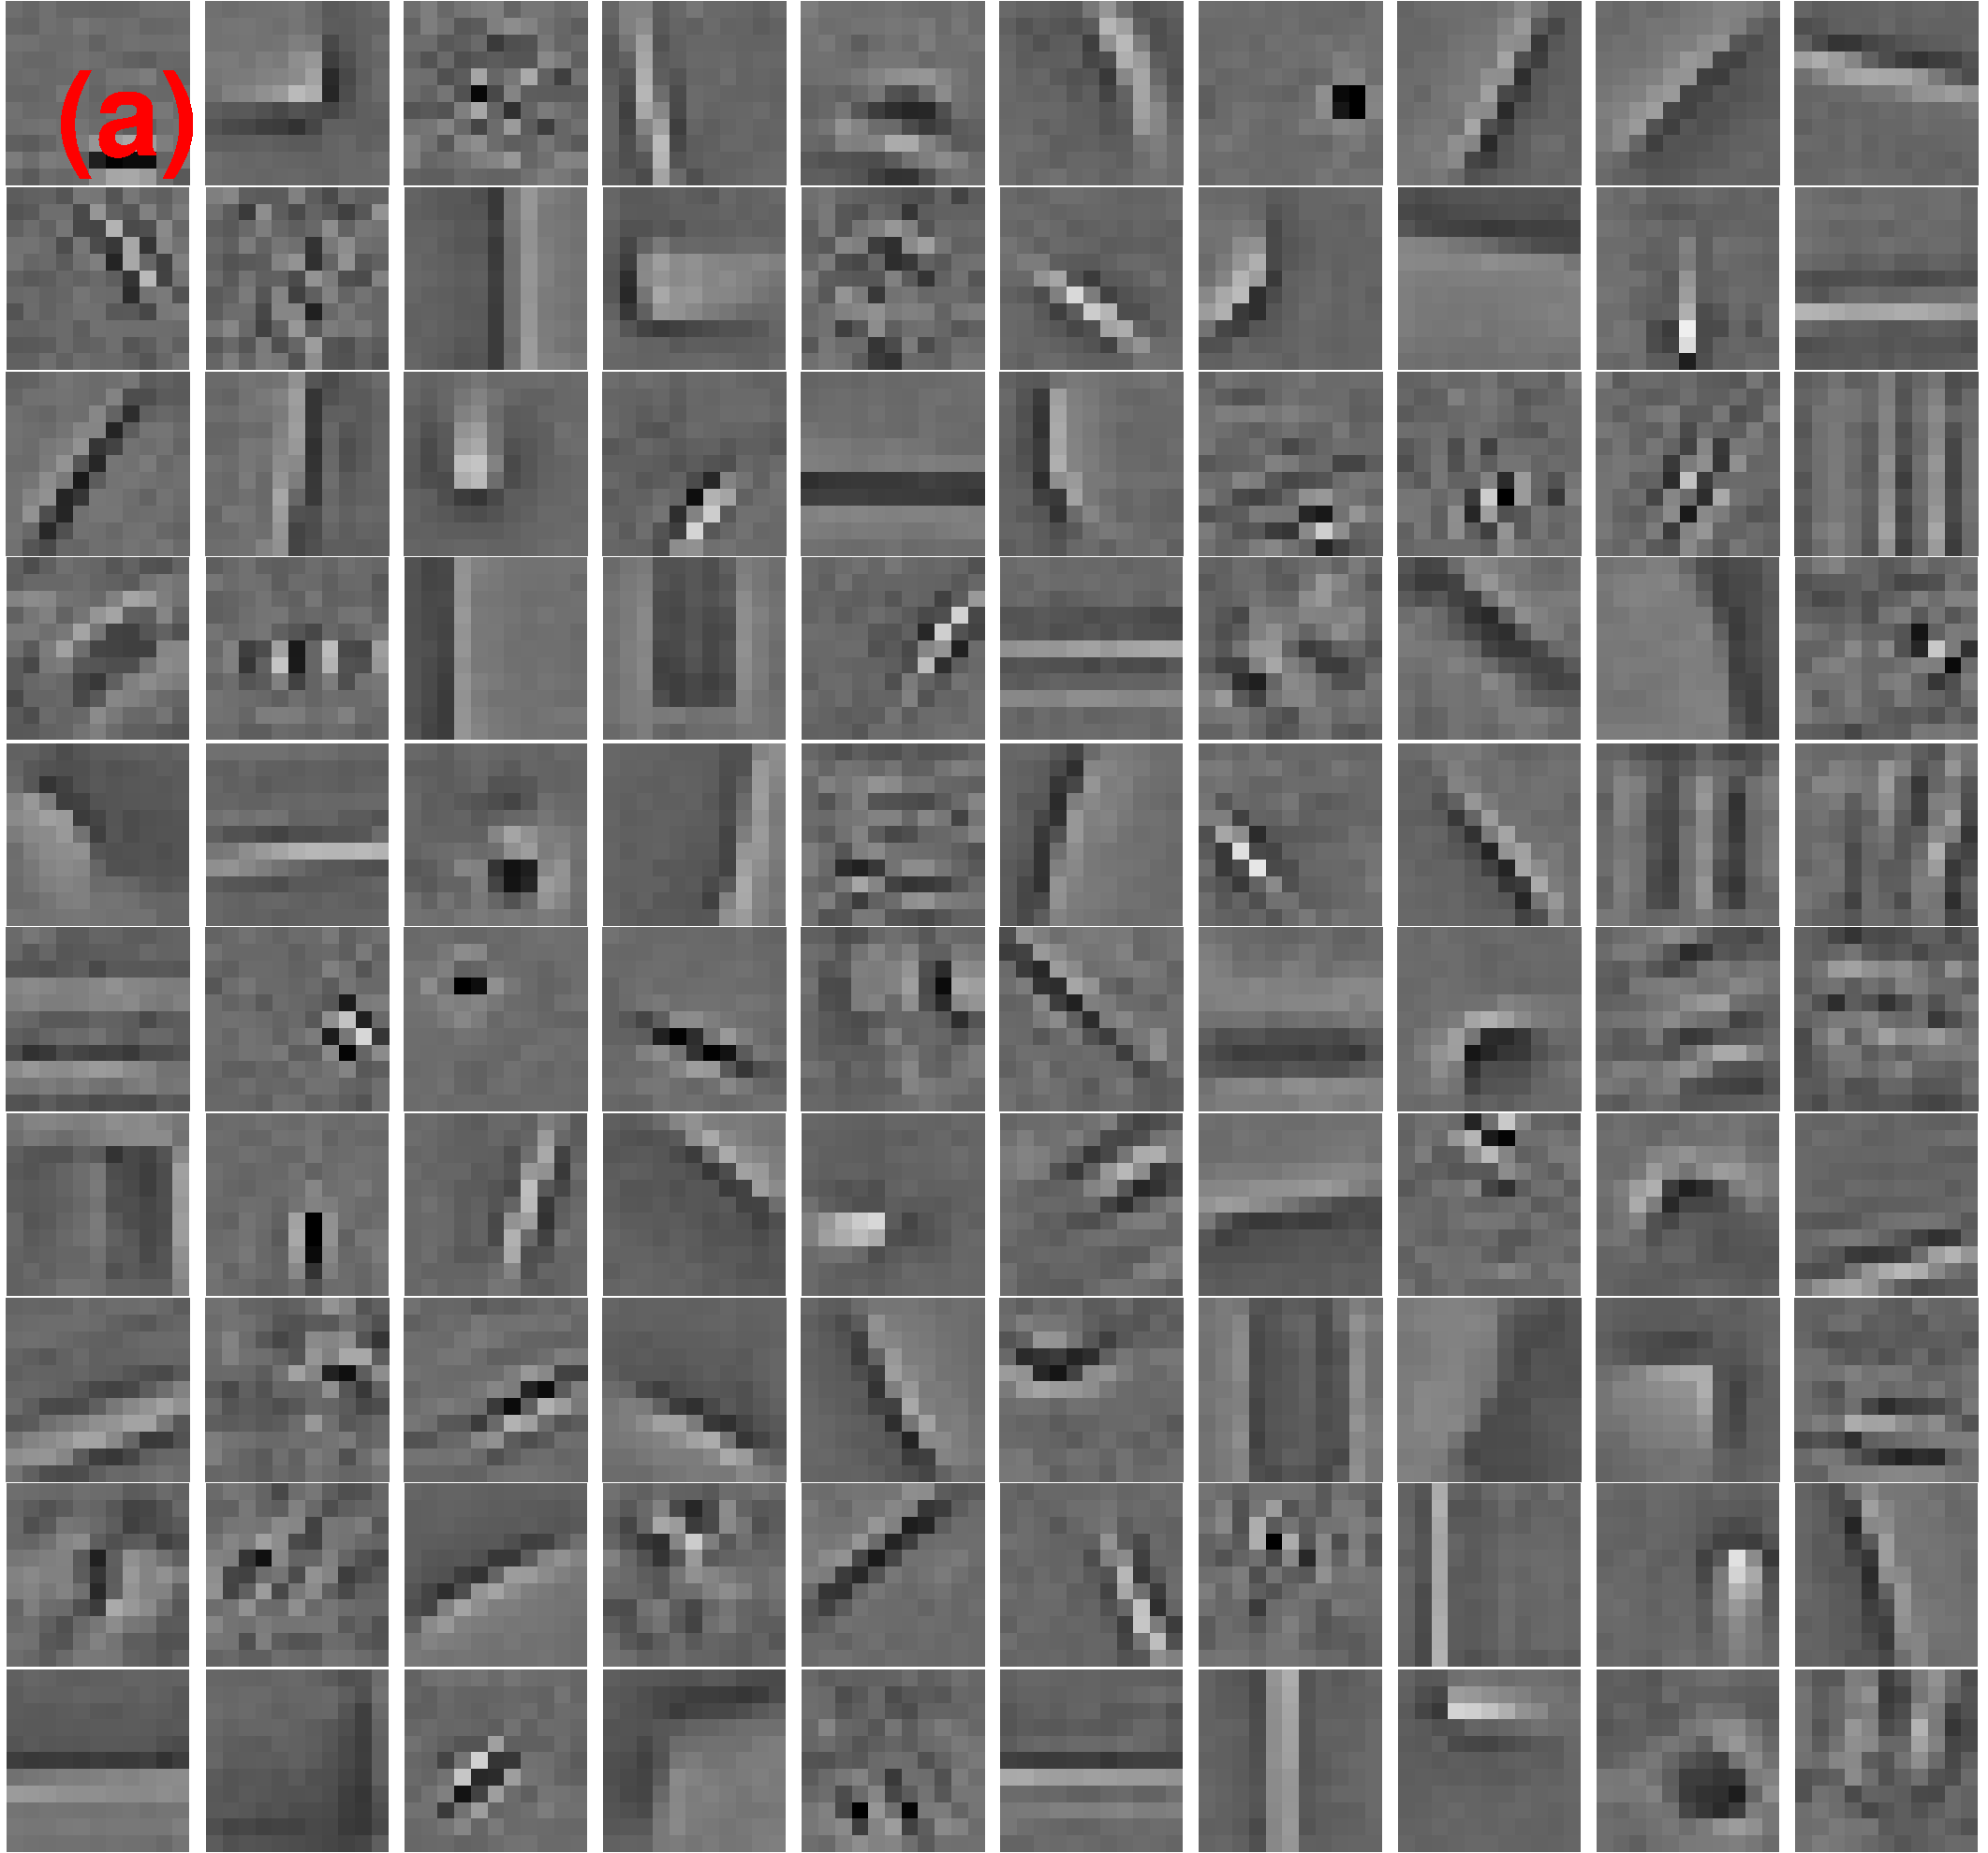
\includegraphics[width=0.75\linewidth]{figure/liu100-filter.pdf}
  \vspace*{2mm}
\end{subfigure}

\begin{subfigure}{1\textwidth}
    \centering
  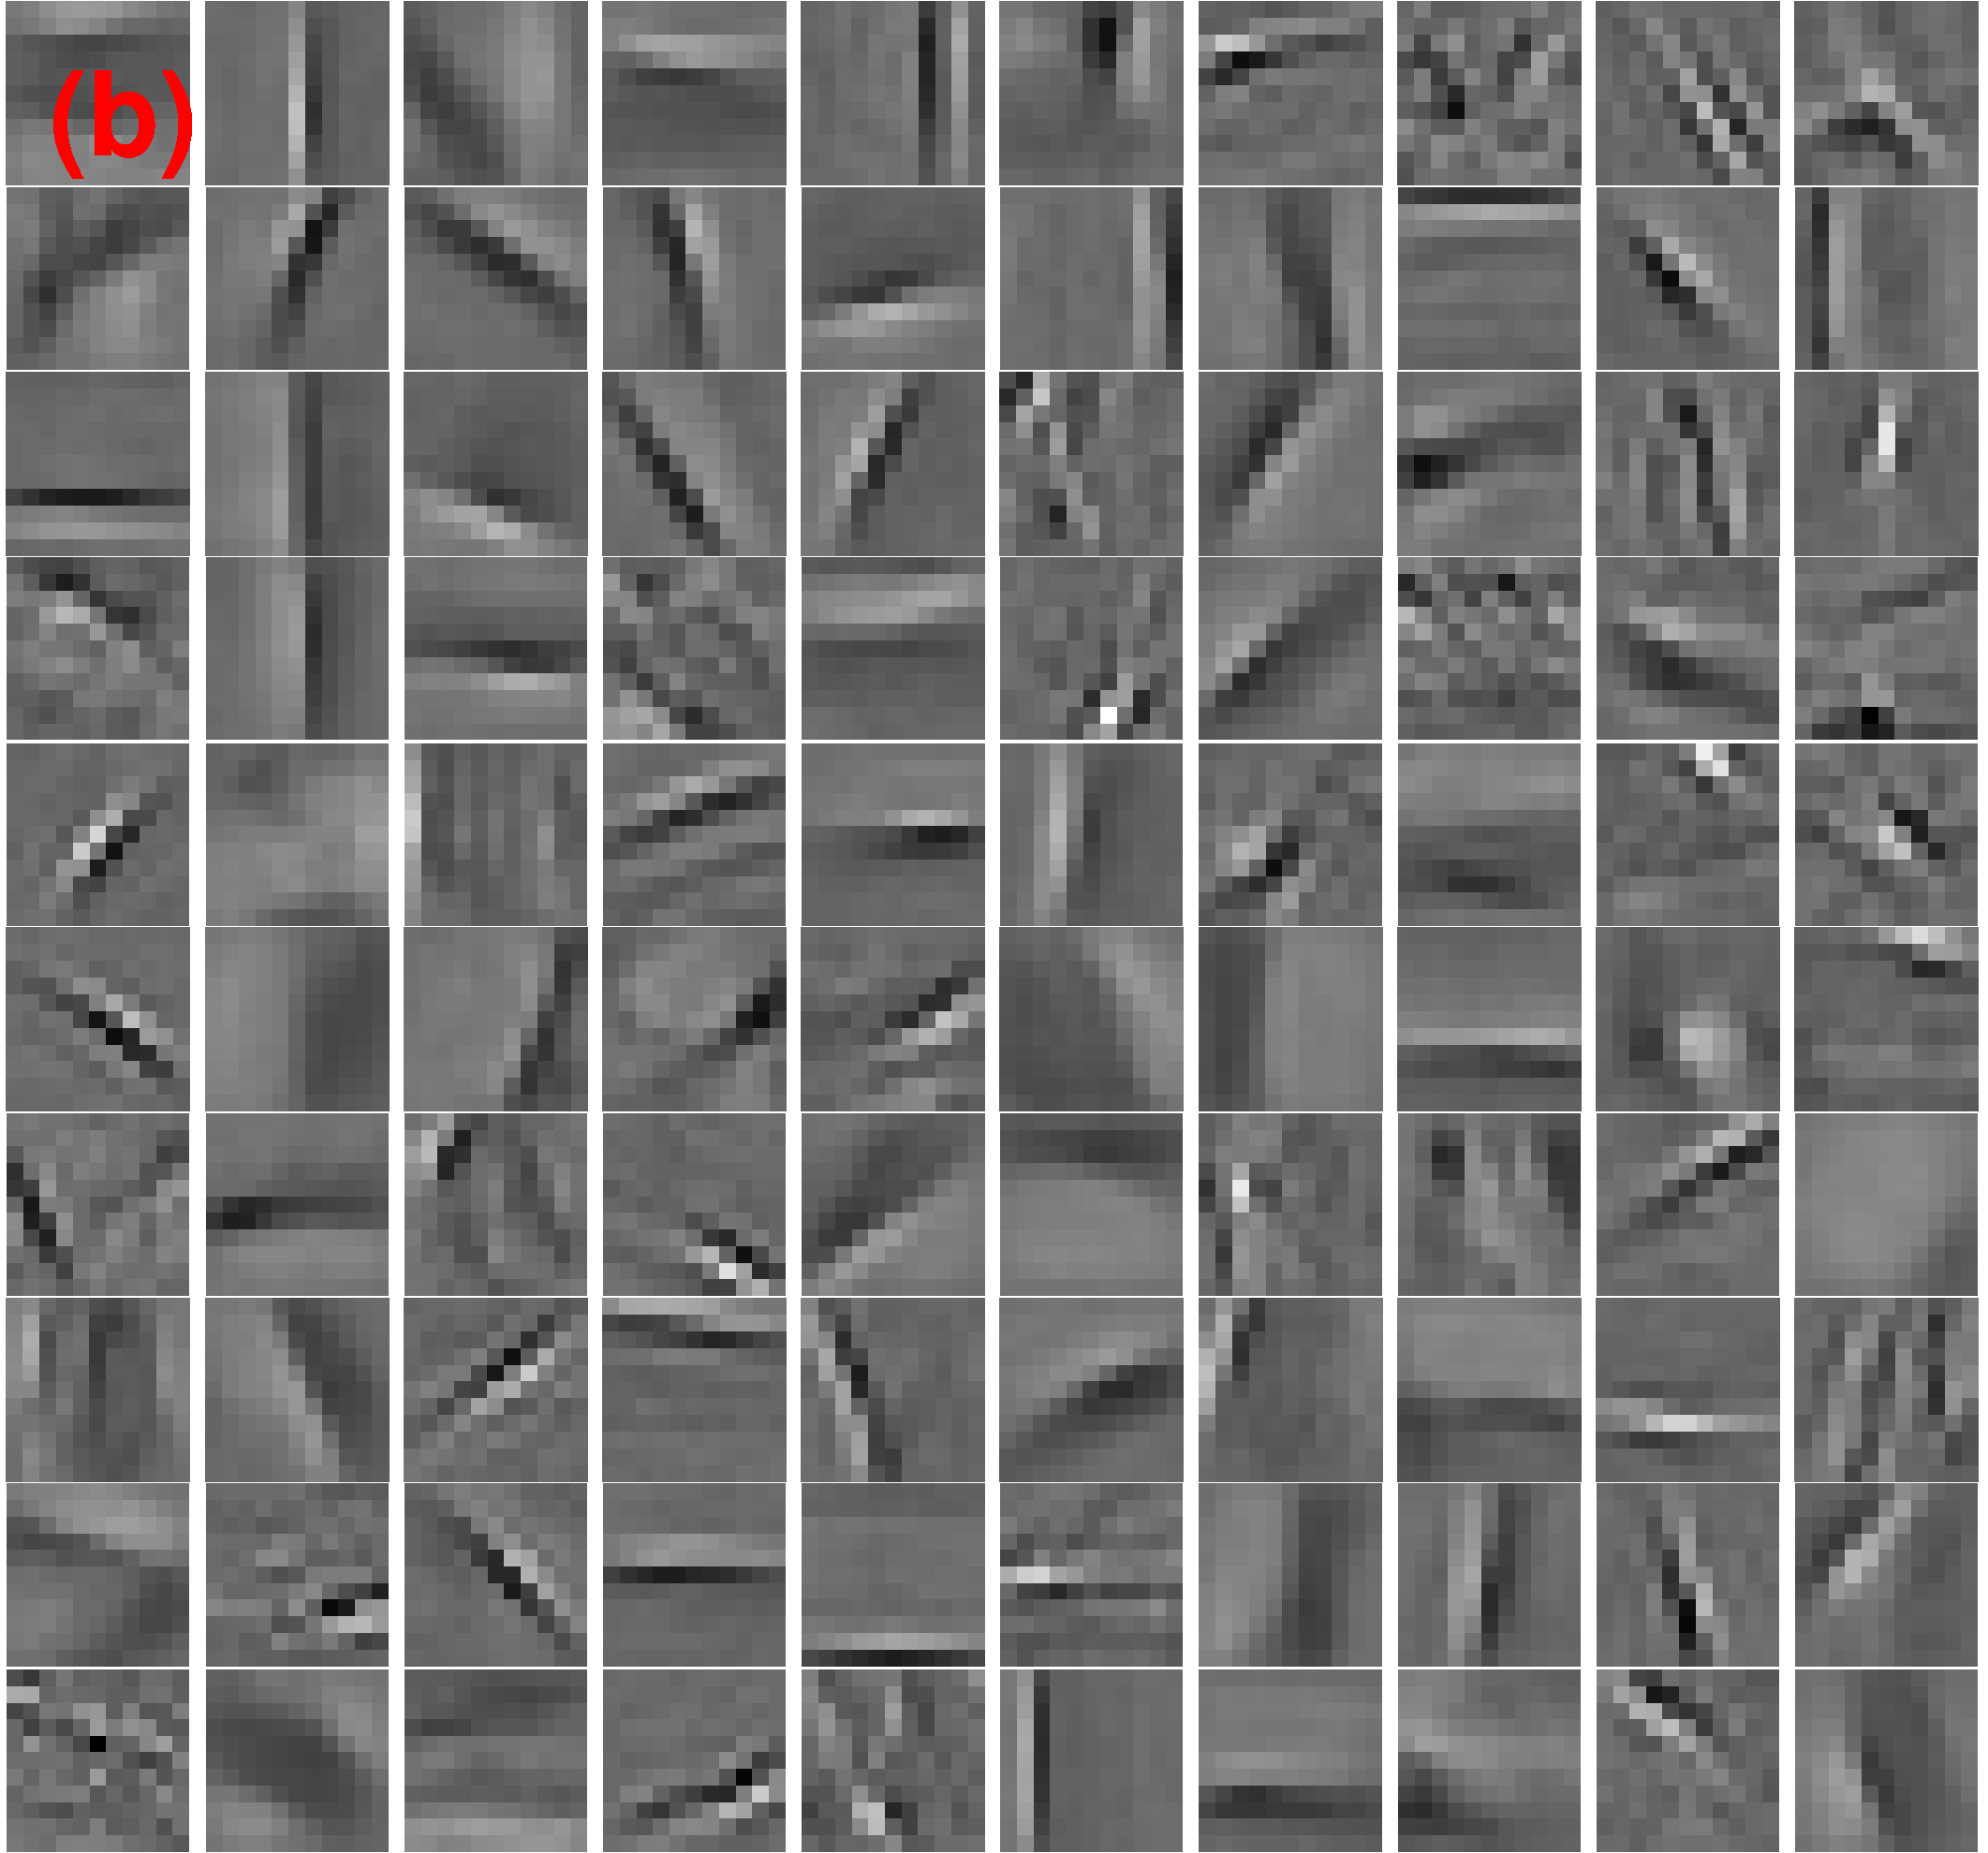
\includegraphics[width=0.75\linewidth]{figure/online100-filter.pdf}
\end{subfigure}
\end{minipage}
\begin{minipage}{0.6\textwidth}
\centering
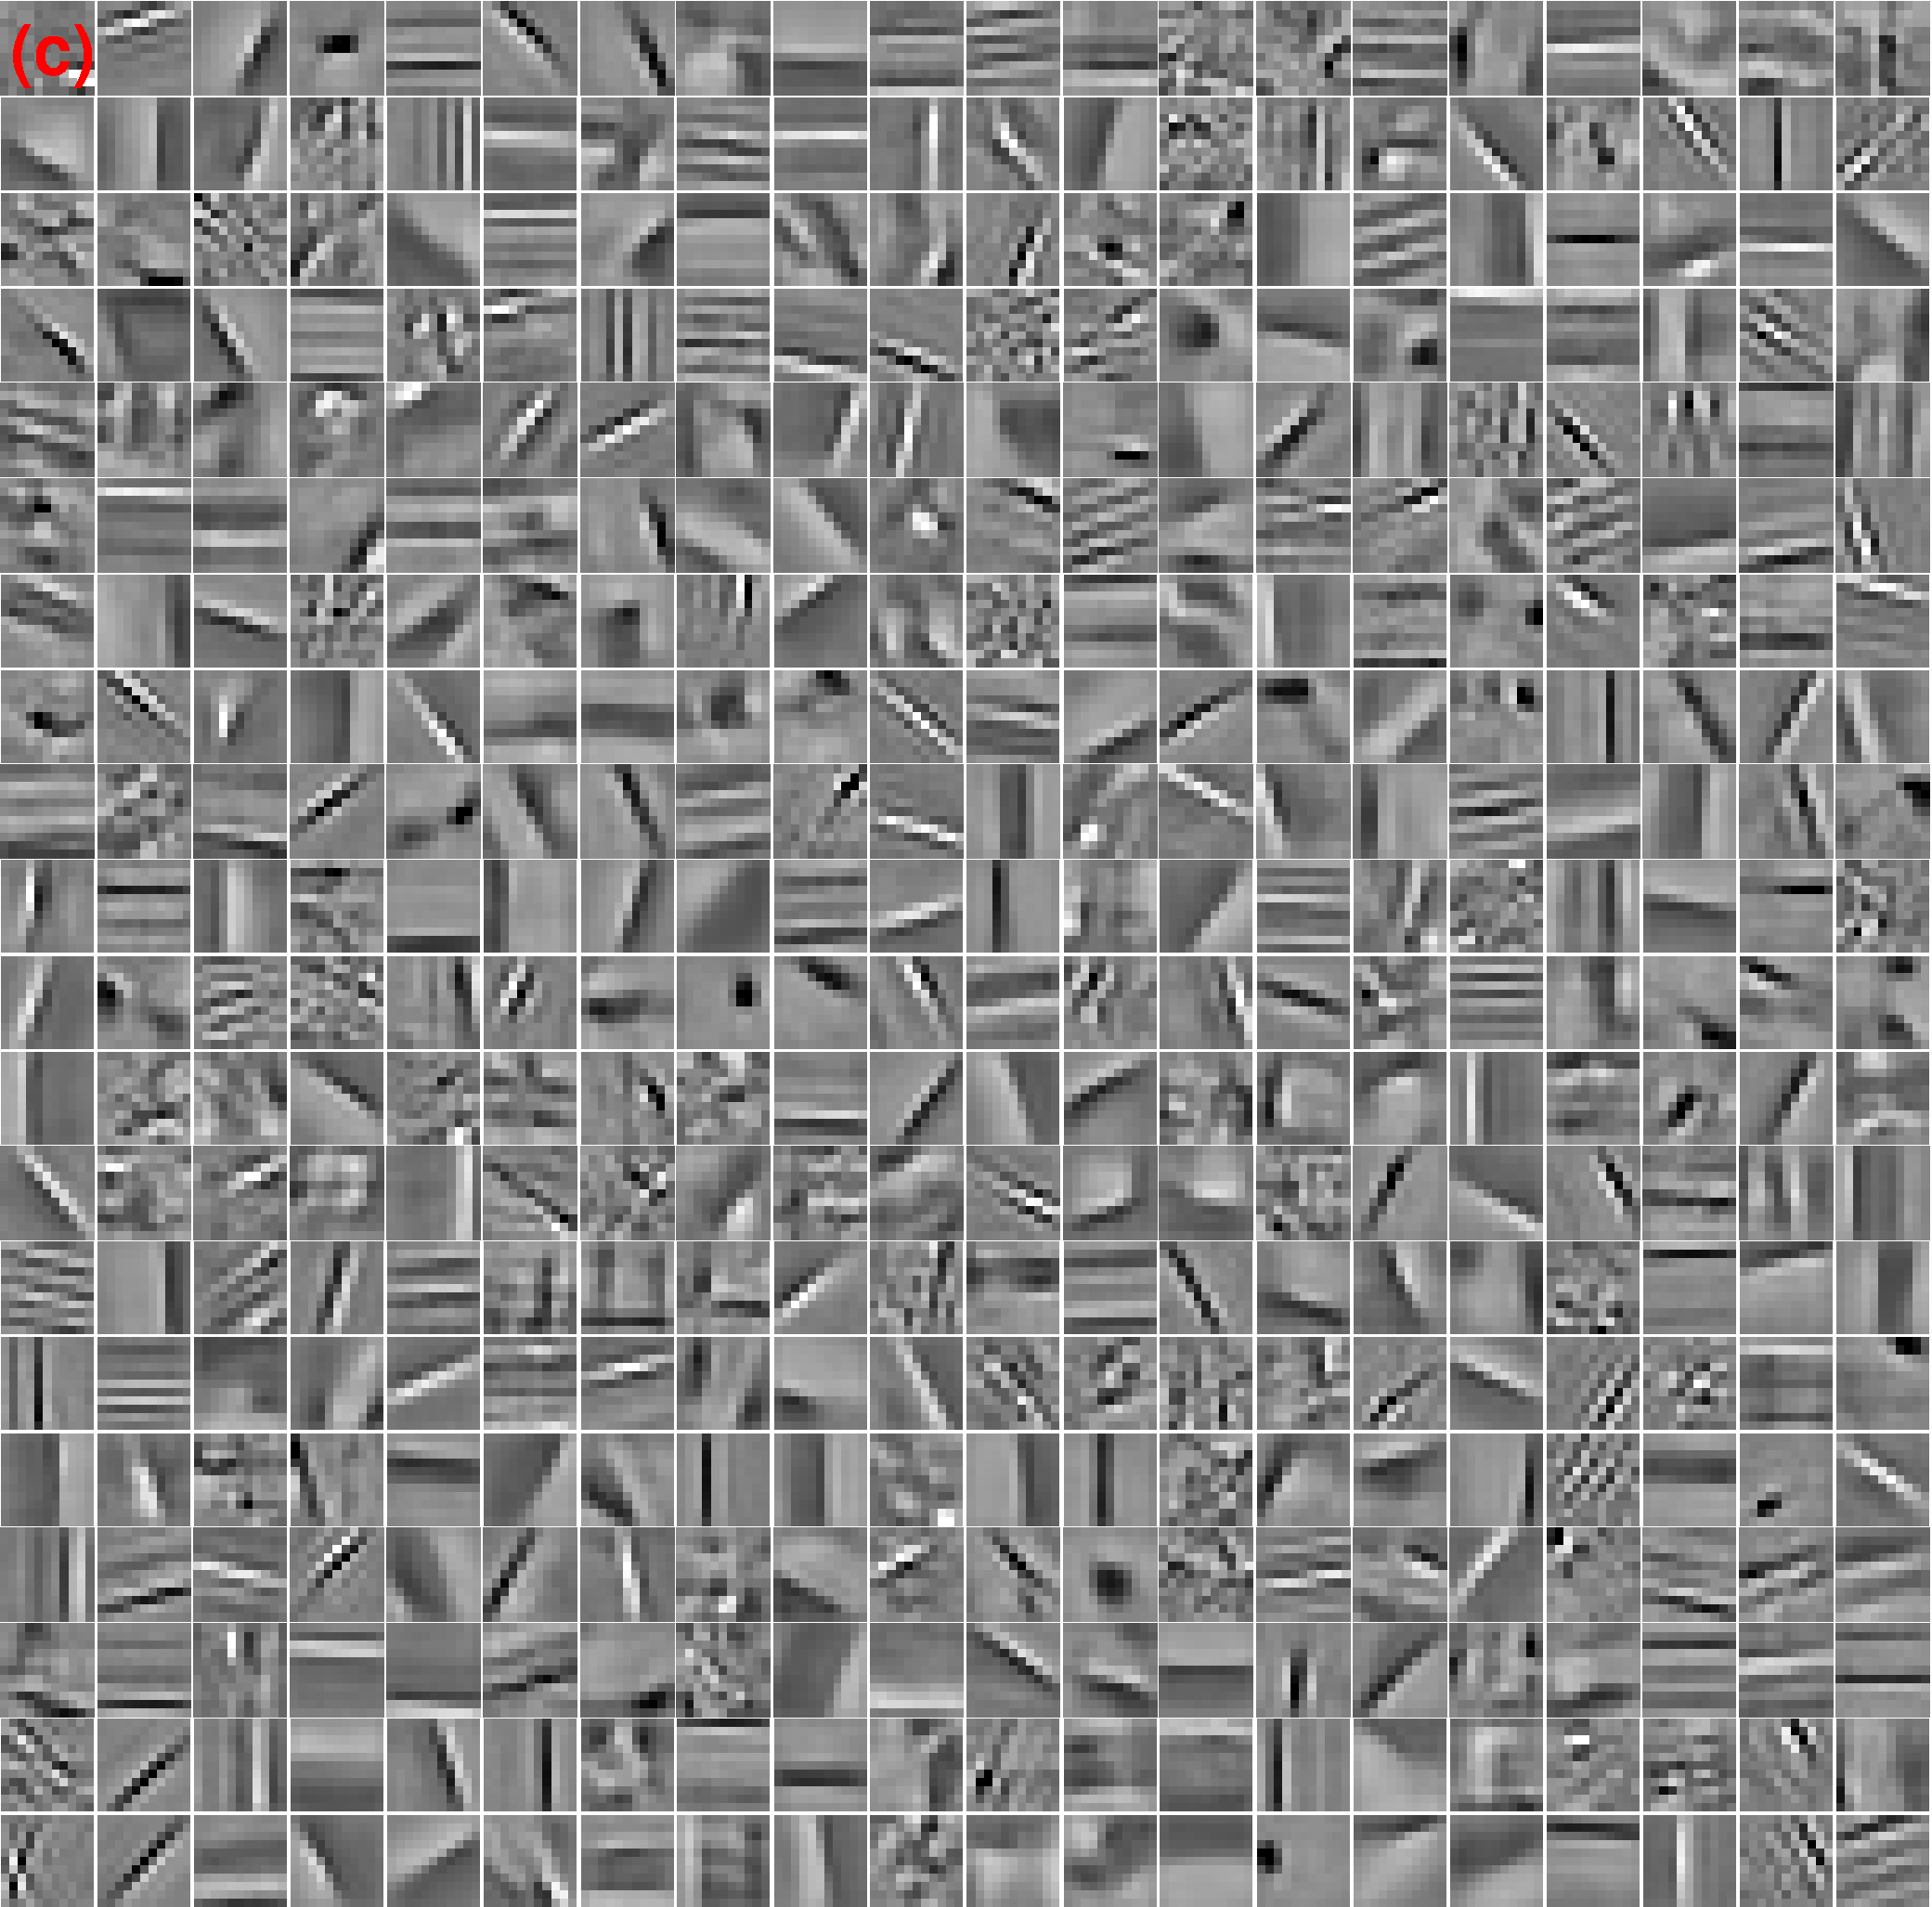
\includegraphics[width=0.97\linewidth]{figure/online400-filter.pdf}
\vspace*{2mm}
\end{minipage}
\begin{minipage}{1\textwidth}
    \centering
    \resizebox{0.8\linewidth}{!}{
        \begin{tabular}{|c||c|c|c|c|c|c|c|c|c|c|}
            \cline{1-11}
            Image & 1 & 2 & 3 & 4 & 5 & 6 & 7 & 8 & 9 & 10 \\
            \hline
            PSNR by (a) & 29.58 & 28.19 & 29.44 & 29.63 & 28.89 & 29.33 & 28.13  & 30.14 & 27.42 & 30.89 \\
            \hline
            PSNR by (b) & 29.63 & 28.22 & 29.57 & 29.90 & 29.12 & 29.59 & 28.05  & 30.17 & 27.53 & 31.08 \\
            \hline
            PSNR by (c) & \textbf{30.24} & \textbf{28.34} & \textbf{29.95}  & \textbf{30.30} & \textbf{29.43} & \textbf{29.96} & \textbf{28.24} & \textbf{30.57} & \textbf{27.72} & \textbf{31.67} \\
            \hline
        \end{tabular} }
\end{minipage}
\caption{Filters learned from 1000 images by our method (SOCSC) and the state-of-the-art online method~\cite{liu-2018-first}, and their corresponding reconstruction quality using the same hyperparameter settings as in Fig.\ \ref{fig:PSNRrecon}. (a) The under-complete dictionary ($11 \times 11 \times 100$) learned by~\cite{liu-2018-first}; (b) The under-complete dictionary ($11 \times 11 \times 100$) learned by SOCSC. (c) The over-complete dictionary ($11 \times 11 \times 400$) learned by SOCSC. These under-complete dictionaries, mainly composed of Gabor-like filters, can be seen as a subset of the represented over-complete dictionary, which contains a number of extra low contrast image features.}
\label{fig:overCompleteDic}
\end{figure*}

{\bfseries Mini-batching.} In practice, a mini-batching strategy would be preferred in order to gain advantages from modern parallel computing architectures. This is also a standard extension to stochastic optimization algorithms~\cite{Takac2013, PCDM, SCSG}. We denote the mini-batch size as $\eta$. In the proposed online algorithm (SOCSC), the time complexity for one step dictionary update will not increase linearly with the increase of $\eta$. Concretely speaking, updating $\code$ is implemented by Cholesky decomposition, and one computation of the matrix factorization can be applied to all of the currently selected batches. Herein, the complexity for doing updating $\code$ $\eta$ times all together is cheaper than $\eta$ times the complexity of updating one $\code$. In addition, the time complexity for updating $\filter$ is not affected by the value of $\eta$, which will be executed only once in each training step regardless of $\eta$. One exception is to update surrogate matrices, the complexity of which is $\eta$ linearly dependent, while this is not dominant in the runtime. The runtime comparisons for various mini-batch sizes are shown in Fig.\ \ref{fig:overComDicAndMinibatch}. Note that larger $\eta$ will result in less number of iterations to process all 1000 images. The plots show that a larger mini-batch size will generally lead to a greater progress in first few training steps, though it takes additional running time and memory. Overall, mini-batched updates provides a more runtime efficient learning process in the online-based CSC model, and according to the obtained experimental results, $\eta=20$ achieves one magnitude speedup over $\eta=1$ to reach a condition with the same level convergence on a single-core program. Since computing sparse codes is a data-independent process, this mini-batched approach can be further accelerated by a distributed computing system.
\begin{figure}[h]
\centering
\begin{subfigure}{0.5\textwidth}
  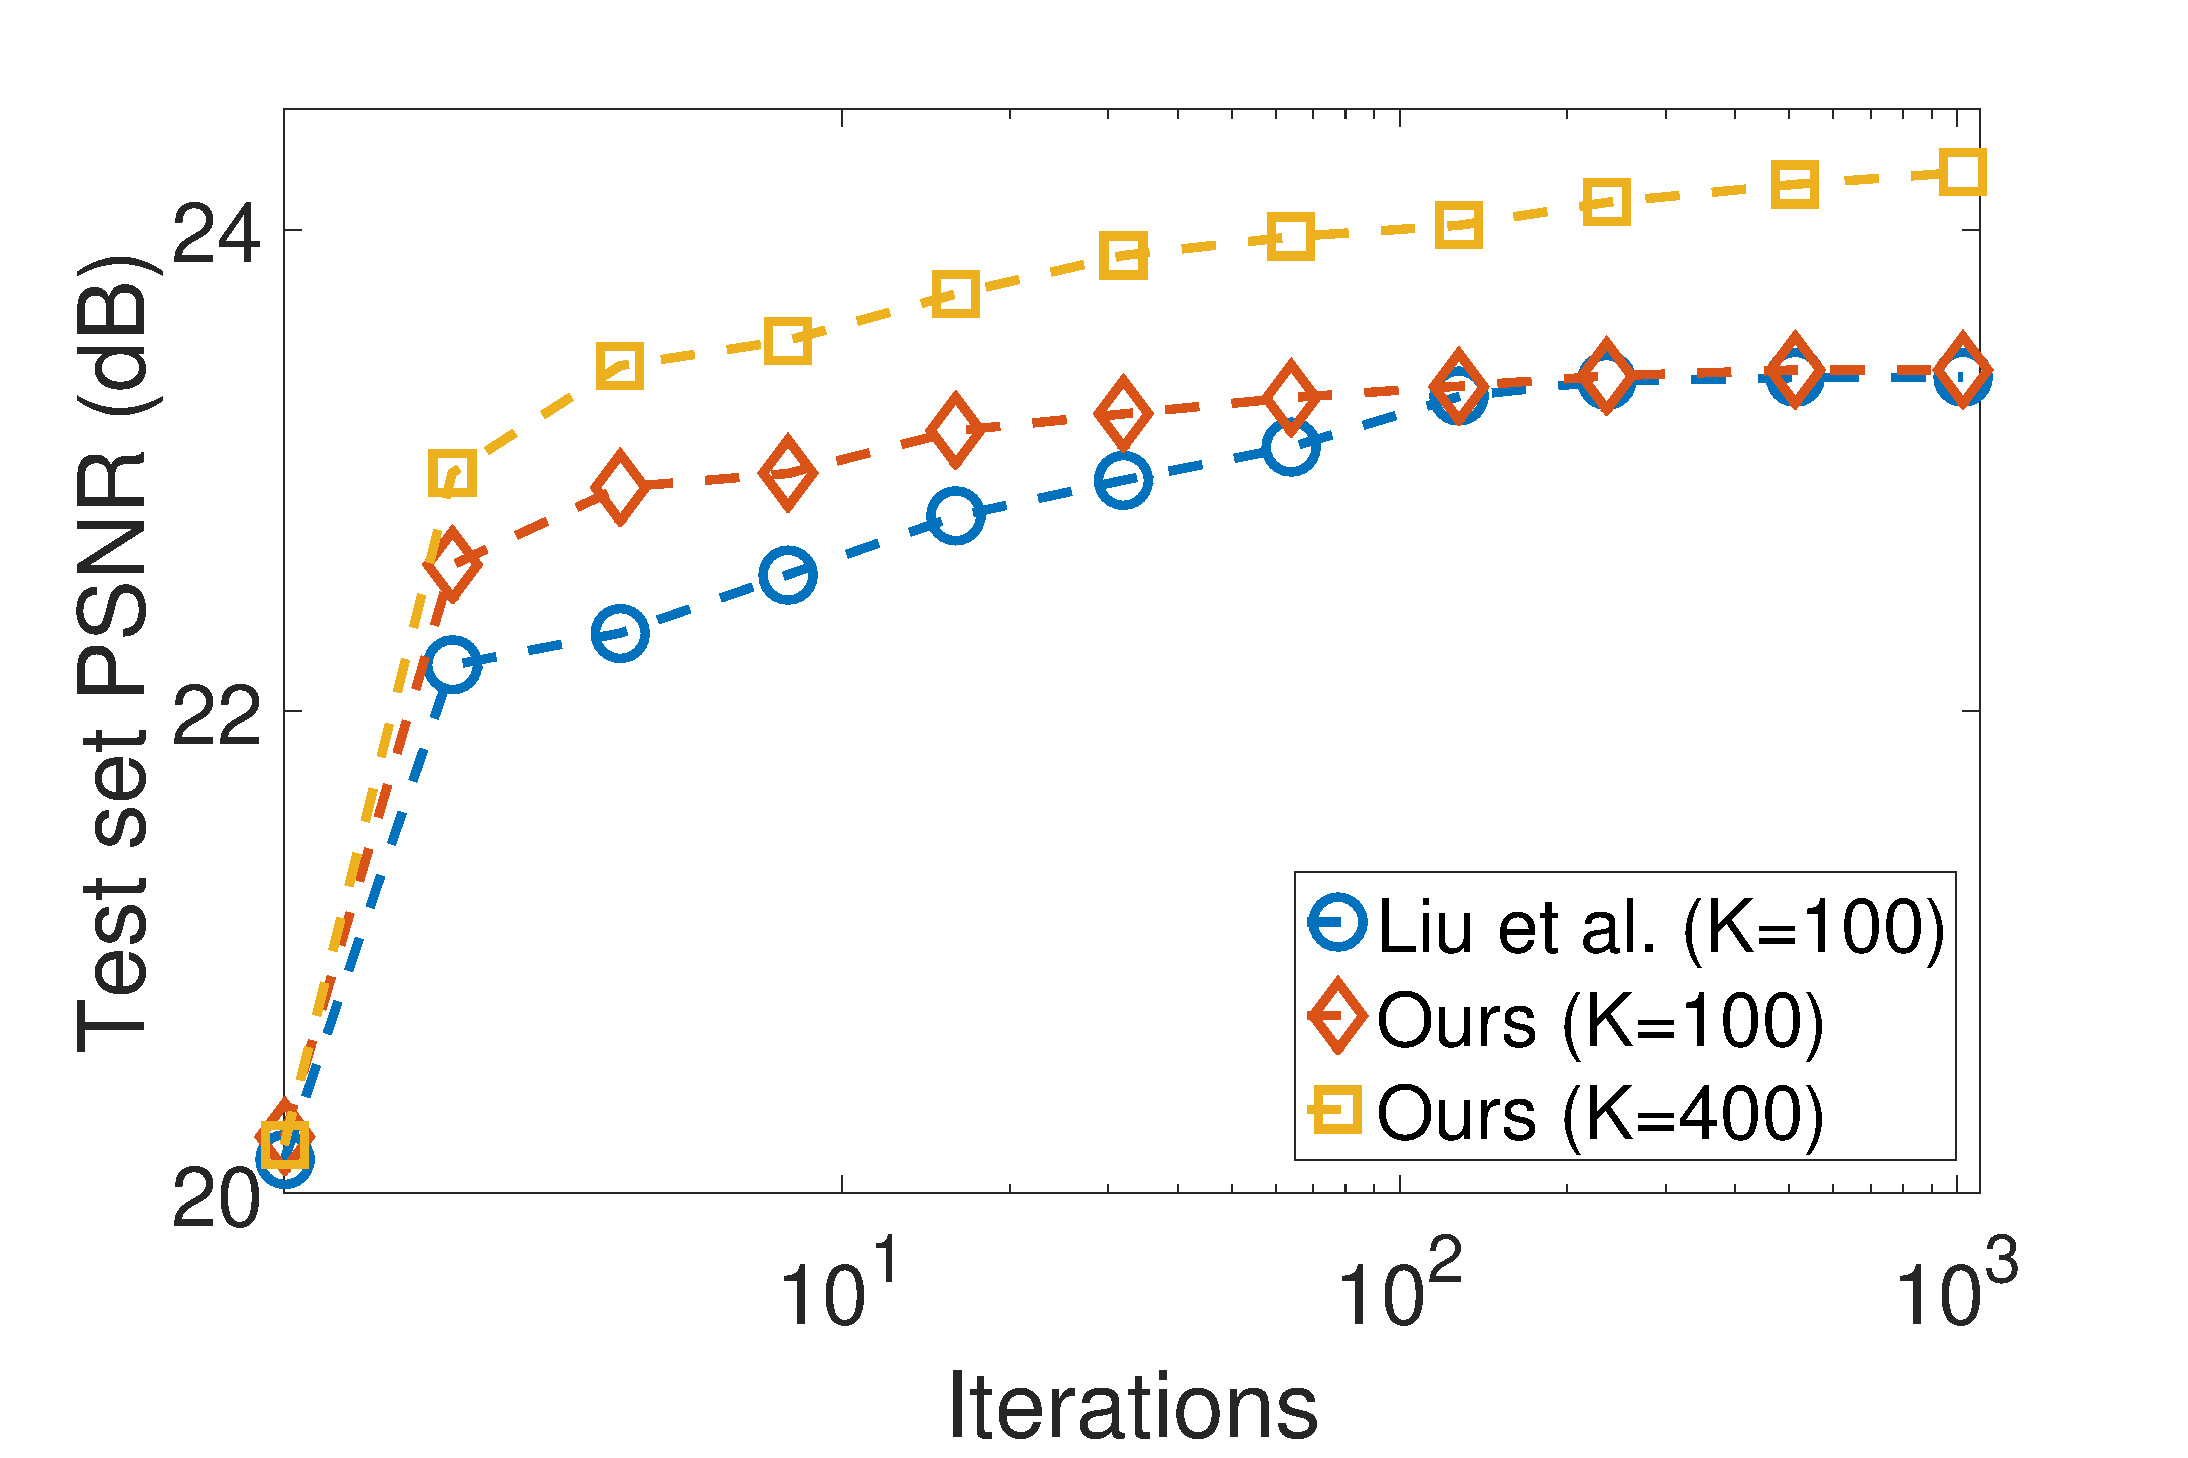
\includegraphics[width=1\linewidth]{figure/overComplete-ite.pdf}
\end{subfigure}
\begin{subfigure}{0.5\textwidth}
  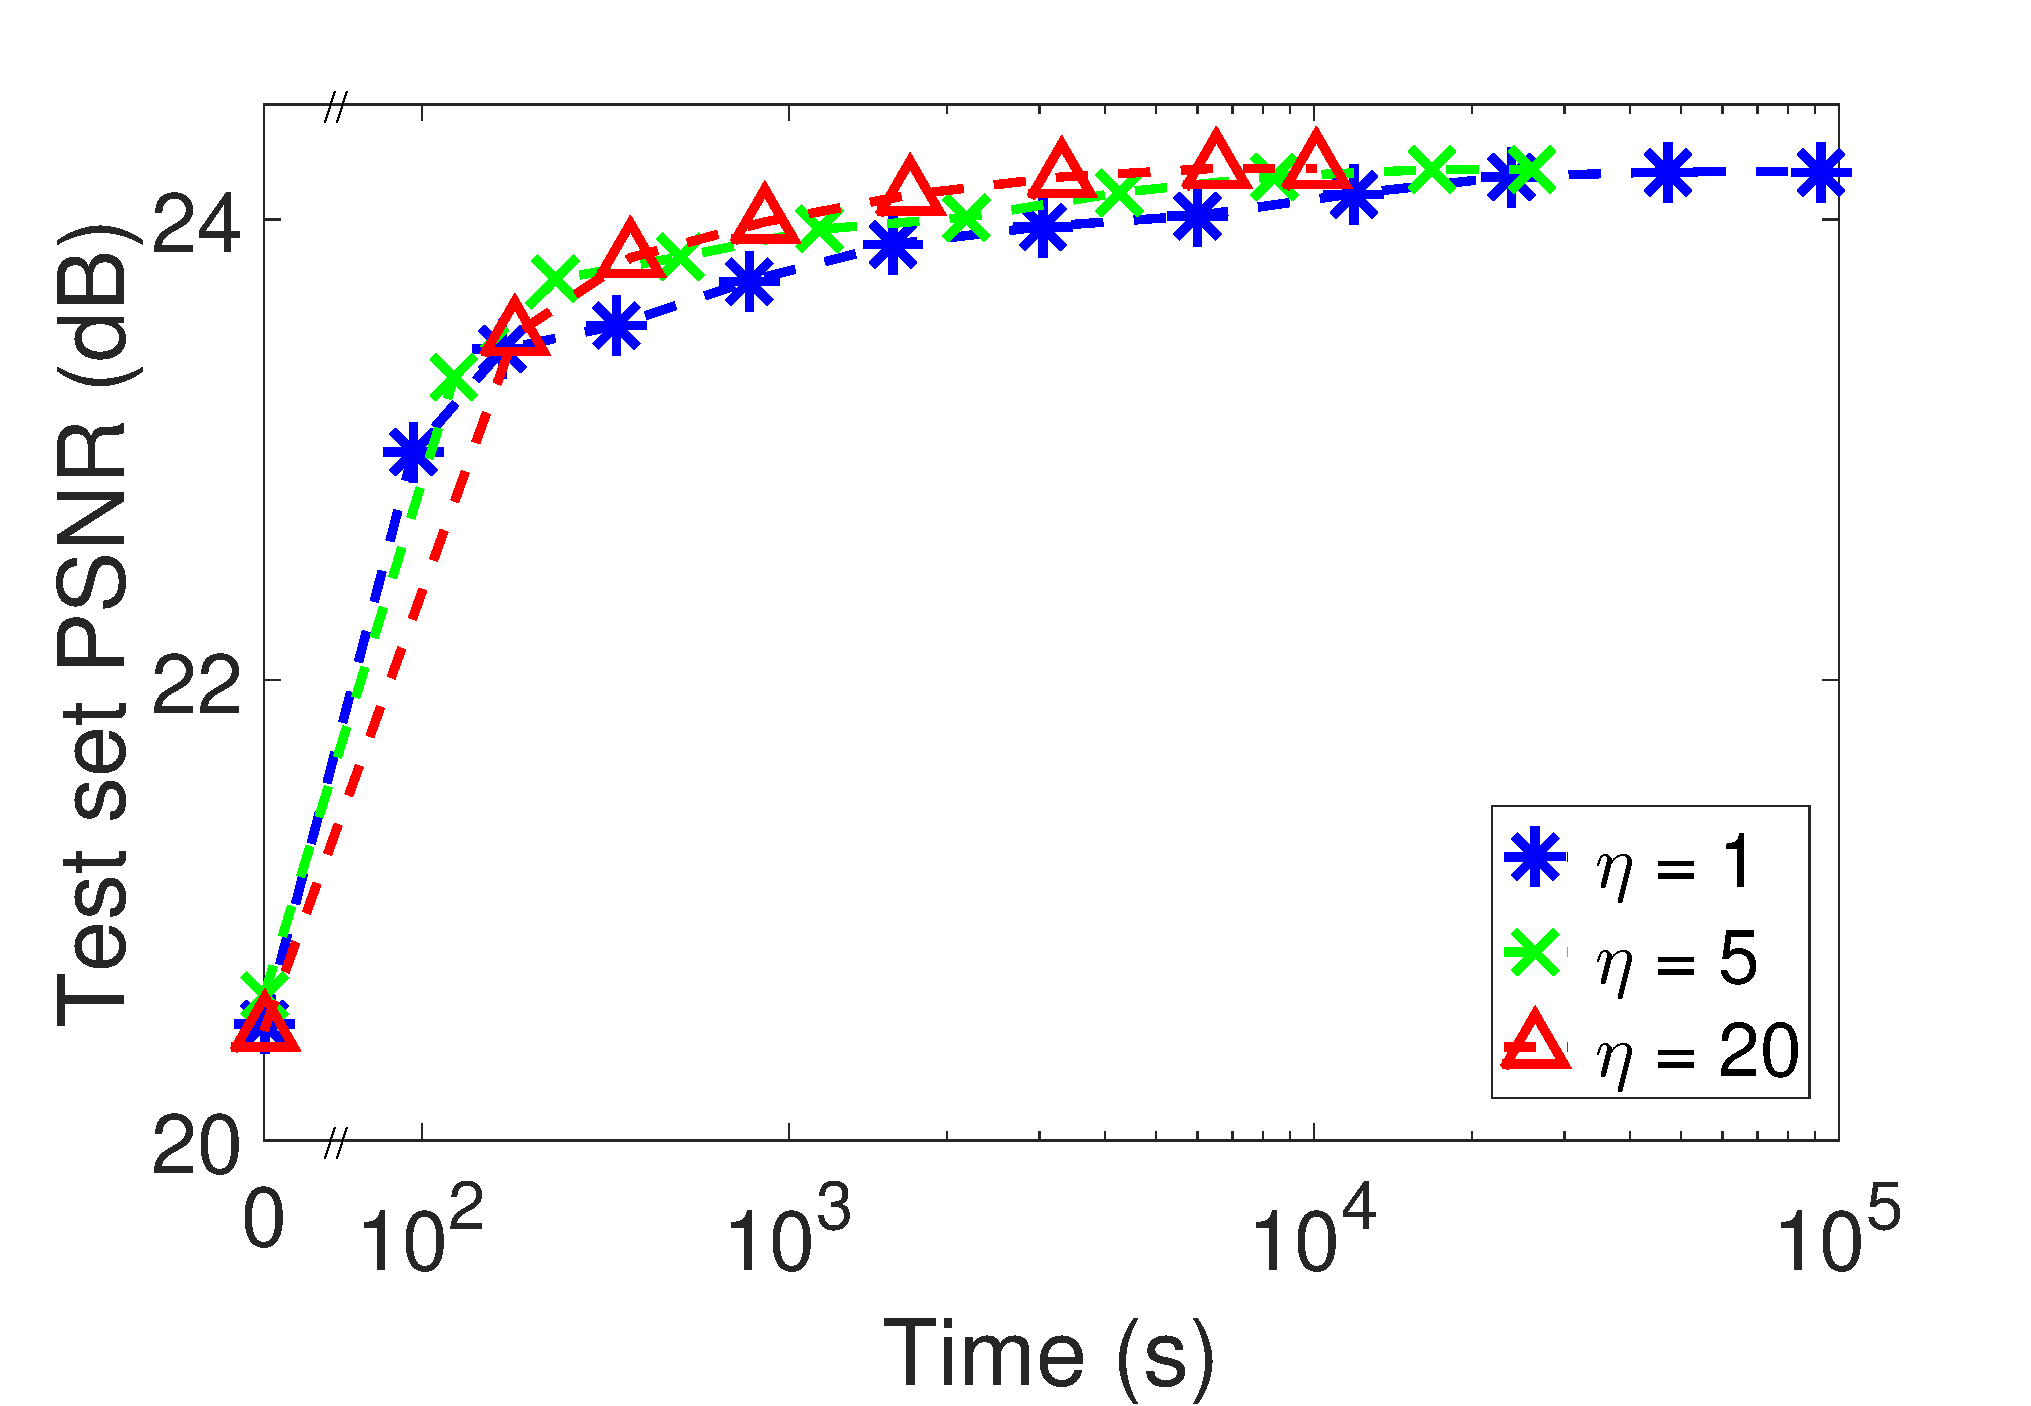
\includegraphics[width=1\linewidth]{figure/minibatch.pdf}
\end{subfigure}

\caption{Top: Testing PSNR for the comparable method~\cite{liu-2018-first} with $K=100$, and our method (SOCSC) with $K=100$ and $K=400$, respectively. Every iteration draws a single image from those 1000 image patches. Bottom: Testing PSNR for SOCSC ($K=400$) with varying values of $\eta$. The learned filters are examined on the test sets every $2^i$ iterations and also at the last iteration, where $i=0,1,\dots$. Note that all the results are generated by a single-core program.}
\label{fig:overComDicAndMinibatch}
\end{figure} 